\documentclass[journal,twoside,web]{IEEEtran}
\usepackage{amsmath,amssymb,graphicx,booktabs,array,tabularx,multirow,url}
\usepackage[T1]{fontenc}
\usepackage{newtxtext,newtxmath}
\usepackage{microtype}
\usepackage{algorithm,algpseudocode}
\floatstyle{boxed}\restylefloat{algorithm}
\usepackage{placeins,dblfloatfix}
\usepackage[hidelinks]{hyperref}
\hypersetup{pdfauthor={Wasil Kayani and Umar Asghar},pdftitle={Explainable Visual Analytics and Forensic Shortcut Auditing of Human and Diffusion Artwork Across Art-Historical Movements}}
\graphicspath{{figures/}}
\newcolumntype{Y}{>{\raggedright\arraybackslash}X}
\setlength{\textfloatsep}{9pt plus 2pt minus 2pt}
\setlength{\dbltextfloatsep}{7pt plus 1pt minus 1pt}\setlength{\dblfloatsep}{5pt plus 1pt minus 1pt}
\setlength{\floatsep}{8pt plus 2pt minus 2pt}
\setlength{\intextsep}{8pt plus 2pt minus 2pt}
\hyphenation{AI-ArtBench Wasser-stein}
\setcounter{dbltopnumber}{4}
\setcounter{topnumber}{4}
\setcounter{totalnumber}{6}
\renewcommand{\dbltopfraction}{0.92}
\renewcommand{\topfraction}{0.92}
\renewcommand{\textfraction}{0.06}
\renewcommand{\floatpagefraction}{0.8}
\renewcommand{\dblfloatpagefraction}{0.8}
\title{Explainable Visual Analytics and Forensic Shortcut Auditing of Human and Diffusion Artwork Across Art-Historical Movements}
\author{\begin{tabular}{@{}c@{\hspace{0.45in}}c@{}}
Wasil Kayani & Umar Asghar\\[3pt]
\normalsize Department of AI \& Data Science & \normalsize Department of AI \& Data Science\\
\normalsize FAST-NUCES, Islamabad, Pakistan & \normalsize FAST-NUCES, Islamabad, Pakistan\\
\normalsize i242551@nu.edu.pk & \normalsize i242532@nu.edu.pk
\end{tabular}}
\linespread{0.97}
\begin{document}
\raggedbottom
\maketitle
\begin{abstract}
Diffusion-artwork detection can rank benchmark origins accurately without isolating which differences survive source confounds. This study combines named image measurements, grouped evaluation, projection diagnostics and a common-support gate. An exhaustive AI-ArtBench audit covers 185,015 files; a balanced tier contains 45,000 artworks, including a native-$256^2$ Human--Latent Diffusion primary cohort of 30,000 with 6,000 held-out test images. A 104-feature handcrafted logistic probe attains area under the receiver operating characteristic curve (AUROC) 0.9824 and F1, the harmonic mean of precision and recall, 0.9420. It trails frozen ResNet-50 (0.9999) and DINOv2 (0.9997), while exceeding the internal fast Fourier transform (FFT)-only comparator by 0.2985 AUROC. Of 1,040 within-style feature comparisons, 542 meet an exploratory statistical rule. Metadata AUROC 1.0000 reveals origin-aligned technical information, but JPEG common support and verified subject matches are absent; no comparison is eligible for confirmatory diffusion-origin attribution. Removing ordinal features reduces AUROC by 0.0744 to 0.9080; JPEG-quality-50 recompression reduces it to 0.6819. Linked artwork views and measured projection fidelity make these associations inspectable. The contribution is a descriptive atlas and a negative validity audit, not confirmation of an encoding-independent origin effect.
\end{abstract}
\begin{IEEEkeywords}
Computational Aesthetics, Explainable Visual Analytics, Diffusion Artwork Detection, Complexity--Entropy Plane, Shortcut Learning Audit, Wasserstein Style Drift.
\end{IEEEkeywords}
\bstctlcite{bstctl}

\section{Introduction}
Artwork provenance affects attribution, collection practice and the credibility of authenticity claims. Diffusion images complicate these tasks, while benchmark-specific content or processing can make a detector appear more general than it is \cite{p1,p3}. The practical question is which measured differences reflect origin and which merely identify the dataset. Within-movement analysis therefore requires named measurements and explicit controls.

Within each AI-ArtBench style, the question is which human--diffusion measurement differences survive subject, native-size and encoding controls. \textbf{G1} concerns inspectable diagnostics and projection fidelity; \textbf{G2}, within-style distribution differences; and \textbf{G3}, survival under verified controls. The temporal question was refined before execution: movement labels do not establish chronology or aesthetic intention.

ArtBrain supplies the artwork benchmark \cite{p1}; complexity--entropy analysis supplies inspectable formal coordinates \cite{p2}.

Code and reproducibility artifacts are prepared for the official repository\footnote{\url{https://github.com/wasil-7/explainable-diffusion-art-analytics}}.

The contributions are:
\begin{itemize}
\item An exhaustive 185,015-file audit and frozen grouped splits, separating a 45,000-artwork balanced tier from the 30,000-artwork native-resolution primary comparison.
\item A transparent 104-predictor probe (AUROC 0.9824), trailing ResNet-50 by 0.0175 (95\% interval $[-0.0216,-0.0140]$) and DINOv2 by 0.0173, while exceeding FFT-only, a matched internal ablation comparator, by 0.2985.
\item A control-gated analysis of 1,040 style-feature contrasts: 542 exploratory passes, but zero eligible confirmations because JPEG support and verified subjects are absent.
\item Audited projections, including PCA trustworthiness 0.6928, and paired sensitivity evidence: ordinal removal loses 0.0744 AUROC and JPEG 50 yields AUROC 0.6819.
\item An artwork-linked dashboard and eight-case forensic gallery connecting aggregate results to actual quadrant pixels and cached measurements.
\end{itemize}
Section II synthesizes related work; Section III formulates the method. Section IV describes setup, and Section V interprets results. Section VI compares base papers, Section VII reports ablations, and Section VIII discusses validity and failures. Section IX concludes; Section X provides declarations, followed by references and a compact reproducibility appendix.

\section{Related Work}
\subsection{Artwork Benchmarks and Complexity--Entropy Aesthetics}
ArtBrain \cite{p1} establishes artwork/source prediction, while complexity--entropy coordinates \cite{p2}, historical latent representations \cite{p11} and self-distilled saliency \cite{p16} support formal or contextual description. Their joint-label, observational or context-prediction tasks do not establish matched binary origin effects. This study instead compares named within-style measurements on frozen grouped Human--LD identities. It treats entropy and complexity as descriptors, not aesthetic merit or chronology.

\subsection{Spectral, Wavelet and Color Forensics}
SCADET \cite{p4}, SPAI \cite{p5} and FIRE \cite{p6} establish learned frequency or reconstruction evidence; SIDWA \cite{p14} learns wavelet attention and CoDA \cite{p8} probes color. Different training, crop contexts and domains prevent direct attribution of those scores to our fixed measurements. The present FFT/Haar/color families expose conditional contributions without reproducing these networks. Grommelt et al. \cite{jpeg_bias} demonstrate JPEG/size bias on GenImage; that prior finding motivates encoding checks but does not prove that our pixel probes use the available JPEG association.

\subsection{Alignment, Generalization and Grounding}
B-Free \cite{p3} establishes content-aligned training and VIB-Net \cite{p7} tests detector generalization. FakeBench \cite{p12}, pixel-inconsistency localization \cite{p13} and region reasoning \cite{p15} provide supervised explanations or localization beyond the semantic labels available here. Their photographic, AP, localization and explanation endpoints do not form a matched artwork-AUROC comparison. This study exposes missing subject support explicitly and links release-labeled errors to pixels; it claims neither equivalent content alignment nor unseen-generator performance.

\subsection{Scalable and Diagnostic Visual Analytics}
PixelatedScatter \cite{p9} establishes count-aware display abstraction, while MisVisFix \cite{p10} supports visible chart diagnostics. Their display/user-task evaluations do not establish the fidelity or usefulness of this artwork interface. The present workflow measures neighborhood preservation separately and links fixed-axis views to actual quadrant evidence, without claiming a user-study benefit. Table~\ref{tab:t1} summarizes the sixteen reviewed studies with published years and marked manuscript-version evidence.

\begin{table*}[tb]
\caption{Sixteen reviewed studies by theme (Section II), with published years. $\dagger$: collected manuscript version; publication metadata in References.}\label{tab:t1}
\centering
\fontsize{7.5}{8.6}\selectfont
\setlength{\tabcolsep}{3pt}
\renewcommand{\arraystretch}{1.12}
\begin{tabularx}{\textwidth}{>{\hsize=0.800\hsize\linewidth=\hsize\raggedright\arraybackslash}X>{\hsize=0.225\hsize\linewidth=\hsize\raggedright\arraybackslash}X>{\hsize=1.450\hsize\linewidth=\hsize\raggedright\arraybackslash}X>{\hsize=1.600\hsize\linewidth=\hsize\raggedright\arraybackslash}X>{\hsize=0.925\hsize\linewidth=\hsize\raggedright\arraybackslash}X}
\toprule
\textbf{Study / year / venue} & \textbf{Theme} & \textbf{Dataset and protocol} & \textbf{Reported endpoint} & \textbf{Comparison limit}\\\midrule
{}\cite{p1} ArtBrain / 2026 / IEEE TMM$\dagger$ & A & AI-ArtBench, 185,015; joint source/style and attribution; test reused for validation & Joint F1 0.869; attribution accuracy 0.999 & Joint labels; distinct test protocol\\
{}\cite{p2} Complexity--entropy / 2025 / Sci. Rep. & A & 149,780 platform works, 2010--2020; observational, no origin split & H--C distributions; 149,780 artworks & Platform art; no origin probe\\
{}\cite{p3} B-Free / 2025 / CVPR & C & COCO: 51,517 real, 309,102 generated; aligned training, external tests & DINOv2+reg e2e AUC/BA 99.0\%/95.2\%; probing 80.8\%/68.5\% & Photographs; not this artwork split\\
{}\cite{p4} SCADET / 2025 / PLOS One & B & AI-ArtBench; 7:1:2; full/local and unseen-generator tests & Full/local AUC 0.962/0.801; cross-model accuracy 0.81 & Different split/crop/model\\
{}\cite{p5} SPAI / 2025 / CVPR & B & 13 generators; spectral self-supervision, cross-generator tests & Mean AUC 91.0\% vs. RINE 85.5\% (+5.5 points); SD3 75.9\%, SD1.3 99.6\% & Cross-generator learned detection\\
{}\cite{p6} FIRE / 2025 / CVPR & B & DiffusionForensics; source-specific training and updated generators & Kandinsky3-trained mean AUC 78.1\% vs. 70.5\% & Source-specific trained detector\\
{}\cite{p7} VIB-Net / 2025 / CVPR & C & 15 Table-1 generator columns (17 overall); cross-series testing & Mean AP 95.53\% vs. NPR 89.98\% & AP is not AUROC\\
{}\cite{p8} CoDA / 2026 / TPAMI & B & FakeForm: 62 domains; photographic training, domain shift & Mean accuracy/AP 77.7\%/88.1\% & AP/domain endpoint differs\\
{}\cite{p9} PixelatedScatter / 2026 / TVCG$\dagger$ & D & Scatterplot datasets; visualization user tasks & E1 Friedman p: 0.0362 / 0.0625 / 0.1070 (600$^2$ / 1200$^2$ / 1800$^2$) & Display study; not embedding fidelity\\
{}\cite{p10} MisVisFix / 2026 / TVCG$\dagger$ & D & Misleading-chart benchmark; chart/user studies & 96\% issue identification; 74 misinformation types & Chart issues; not image authenticity\\
{}\cite{p11} Art evolution / 2026 / PNAS$\dagger$ & A & 72,447 WikiArt works; creation-year regression & Creation-year R$^2$ = 0.869 & Year regression; no AI-origin test\\
{}\cite{p12} FakeBench / 2025 / TIFS$\dagger$ & C & FakeBench; human and zero/few-shot LMM assessment & Human average accuracy 74.51\% & Human/LMM endpoint differs\\
{}\cite{p13} Pixel inconsistency / 2025 / TPAMI$\dagger$ & C & 12 manipulation datasets; localization and perturbations & 16 representative models on 12 datasets & Localization; not source ranking\\
{}\cite{p14} SIDWA / 2026 / Electronics & B & SIDset 8:1:1; additional GenImage testing & Average accuracy >95\%; 18.2 ms, NVIDIA A100 & SIDset; no matched style inference\\
{}\cite{p15} Locate--then--examine / 2026 / arXiv$\dagger$ & C & TRACE; 20,000 region-annotated real/generated examples & 20,000 region-annotated images & Region labels absent here\\
{}\cite{p16} Self-distilled artwork / 2026 / Sci. Rep. & A & Balanced artwork dataset; 70:30; global/local learned detector & Abstract accuracy 99.01\%, precision 95.29\%, recall 94.58\%, F1 94.93\%, AUC 99\% & Different split; abstract metrics scoped\\
\bottomrule\end{tabularx}
\end{table*}

\section{Proposed Methodology}
\subsection{Formulation and Architecture}
An artwork record is $(I_i,y_i,s_i,g_i,m_i)$: RGB image $I_i$, origin label $y_i$ (Human $=0$, LD $=1$ for the primary task), style $s_i$, recorded source-family group $g_i$, and technical metadata $m_i$. The four disjoint $128\times128$ quadrants $\mathcal Q(I_i)=\{q_1,q_2,q_3,q_4\}$ tile each native-$256^2$ canvas once. Groups define the dependence structure. The architecture in Fig.~\ref{fig:f1} freezes IDs and development calibration before descriptive projections and probe evaluation. It explicitly separates origin ranking from eligibility for independent origin attribution.
\begin{figure}[t]

\centering

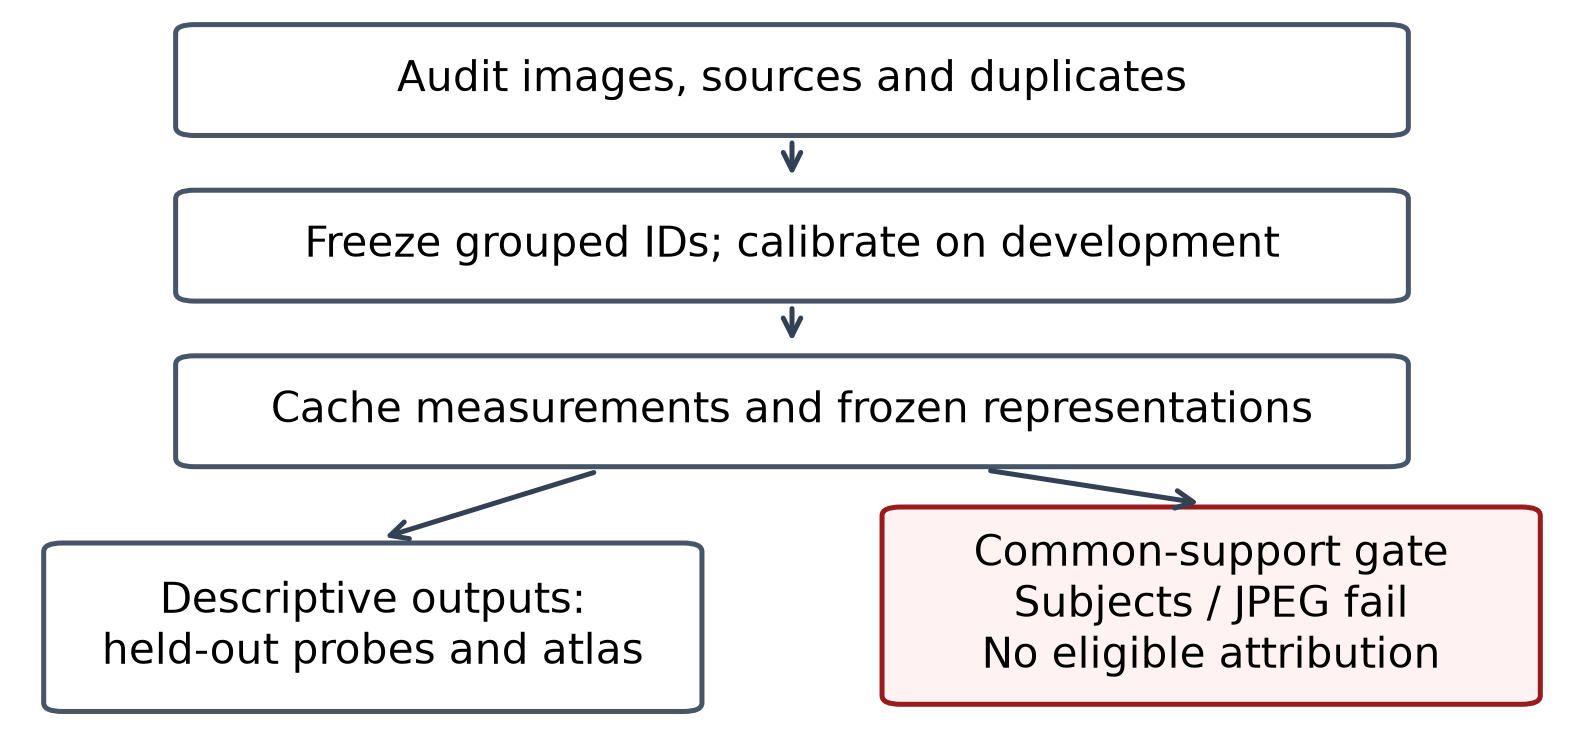
\includegraphics[width=\columnwidth,height=1.55in,keepaspectratio]{figure_01.png}

\caption{Implemented branch structure. Frozen splits and development calibration precede held-out evaluation; descriptive outputs remain available when the common-support gate blocks independent attribution.}\label{fig:f1}

\end{figure}

Algorithm~\ref{alg:pipeline} implements the planned twelve-step workflow. Planned steps 1--3 map to the input and lines 1--3/6; step 4 to lines 4--7; step 5 to line 8; steps 6--7 to lines 9--10/16; steps 8--9 to lines 11--15; and steps 10--12 to line 16 and the output.

\subsection{Mathematical Features}
Let $Y$ denote normalized crop luminance. For permutation entropy \cite{bandt}, stable row-major ranking within each overlapping $2\times2$ neighborhood yields $4!=24$ ordinal states. Their pooled probability vector is $p=(p_1,\ldots,p_{24})$. With uniform distribution $u$ and point mass $\delta$,
\begin{align}
 S(p)&=-\sum_{j=1}^{24}p_j\ln p_j,\quad H=\frac{S(p)}{\ln24},\\
 J(p,u)&=S((p+u)/2)-\tfrac12 S(p)-\tfrac12 S(u),\\
 C_{\!H}&=H\frac{J(p,u)}{J(\delta,u)}.
\end{align}
Here $C_H$ is Jensen--Shannon statistical complexity \cite{rosso}, denoted $C$ on the atlas; a subscript distinguishes it from logistic regularization below. Zero-frequency entropy terms are zero. Stable ties are retained in the primary analysis, with tie exclusion evaluated separately. An empty tie-excluded sample is undefined.

For the frequency family, $P=|\mathcal F\{(Y-\bar Y)h\}|^2$, where $\mathcal F$ is the two-dimensional FFT and $h$ a separable Hann window. Sixteen annuli cover $0<f\leq0.5$ cycles/pixel, excluding DC. Each band sum is normalized by retained power; high-frequency share sums $f>0.25$. The slope $\beta$ regresses log mean band power on log radial frequency. Two-level periodized orthonormal Haar decomposition \cite{imaging,wavelet} yields $LL_2$ and detail bands $LH_1,HL_1,HH_1,LH_2,HL_2,HH_2$. Squared coefficient sums are divided by total raw-luminance coefficient energy, including $LL_2$; Haar normalization does not subtract the mean.

For hue angle $\theta$, saturation-gated pixels satisfy $S>\tau_S=0.01$. The circular summary is $(\bar c,\bar s,R)$, with $\bar c=\langle\cos\theta\rangle$, $\bar s=\langle\sin\theta\rangle$ and $R=(\bar c^2+\bar s^2)^{1/2}$. Valid-hue fraction, saturation/value medians and interquartile ranges, component correlations, CIE $L^*a^*b^*$ summaries and correlations are retained. Edge density uses the Sobel operator \cite{imaging}: the fraction of normalized magnitudes exceeding the development-frozen threshold $\tau_{\mathrm{edge}}=0.048316767248$. Undefined correlations are flagged and imputed only through development-fitted preprocessing.

Median and interquartile-range crop aggregation, plus pooled ordinal probabilities, produce 104 primary predictors: 8 ordinal, 36 FFT, 14 Haar and 46 color/edge features. The cache contains 169 measurements including full-canvas, tie-excluded and diagnostic fields. Raw hue angles and undefined-count flags are excluded from the primary predictor vector.

\subsection{Probe Objective and Statistical Gate}
For development-standardized feature $\tilde x_i$, coefficients $w$, unpenalized intercept $b$ and $N_d$ development artworks, let $\sigma_i=(1+e^{-(w^\top\tilde x_i+b)})^{-1}$. The executed unweighted scikit-learn \cite{sklearn} L-BFGS objective is
\begin{align}
\mathcal L(w,b)&=-\frac{1}{N_d}\sum_{i=1}^{N_d}\{y_i\log\sigma_i+(1-y_i)\log(1-\sigma_i)\}\nonumber\\
&\quad+\frac{\|w\|_2^2}{2N_d C_{\mathrm{solver}}}.
\end{align}
Thus tabulated $C$ values retain the executed solver scale, rather than an unadjusted averaged-loss penalty.

For feature CDFs $F_H,F_L$, Wasserstein distance \cite{ot} is $W_1=\int_{-\infty}^{\infty}|F_H(x)-F_L(x)|\,dx$ and the two-sample Kolmogorov--Smirnov statistic \cite{ks} is $D=\sup_x|F_H(x)-F_L(x)|$. Signed shifts are median(LD) minus median(Human). Sliced distance $SW_1=128^{-1}\sum_{r=1}^{128}W_1(\langle v_r,X_H\rangle,\langle v_r,X_L\rangle)$ averages fixed unit directions $v_r$ in development-standardized space. Source dispersion uses AI/Human interquartile-range ratios with zero denominators flagged.

Let $G$ indicate satisfied subject, native-size, style, encoding and support controls. A comparison is gate-eligible only when these controls hold; an exploratory pass meets the statistical rule without verified controls. Confirmatory eligibility requires
\begin{equation}
 G\ \wedge\ p_{\mathrm{BH}}<0.05\ \wedge\ W_1>P_{95}^{\mathrm{split\text{-}half}}.
\end{equation}
The Benjamini--Hochberg adjustment \cite{bh} spans all 1,040 prespecified feature/style tests. Each style uses 10,000 whole-source-group label randomizations; the number of AI groups is fixed, while artwork counts can vary. Intervals adapt bootstrap resampling \cite{bootstrap} to 1,000 whole-source-group draws; conditional on frozen fits means preprocessing, coefficients and thresholds stay fixed. Within-origin disjoint group halves yield 2,000 pooled null distances. With subject/encoding exchangeability unverified, adjusted probabilities remain exploratory.
\begin{algorithm}[t]
\caption{Control-gated explainable visual analytics}
\label{alg:pipeline}
\footnotesize\begin{algorithmic}[1]
\Require Images, origin/style metadata, source-family rules, seed 42
\State Decode all files; audit dimensions, encoding and duplicate links
\State Form transitive source/duplicate groups; freeze 60:20:20 IDs
\State Select balanced and native-$256^2$ primary cohorts
\State Calibrate hue/Sobel thresholds on development only
\For{each frozen artwork}
\State Tile four disjoint quadrants; cache ordinal/FFT/Haar/color features
\EndFor
\State Evaluate technical, subject and JPEG common-support gates
\State Fit scalers, PCA and probes using development/validation only
\State Freeze fits/thresholds; evaluate identical held-out IDs
\For{each prespecified style-feature comparison}
\State Compute $W_1$, KS $D$, shift, group interval and split-half null
\State Randomize whole-group labels; adjust the complete test family
\State Output exploratory pass separately from gate-eligible confirmation
\EndFor
\State Link projections, ablations and gallery to cached artwork evidence
\Ensure Predictions, descriptive contrasts, support flags and attribution eligibility
\end{algorithmic}
\end{algorithm}

\subsection{Refinements to the Planned Methodology}
The plan's four disjoint quadrants remain primary; five overlapping crops add a sensitivity, while the full-canvas comparison also changes dimensionality. The planned development calibration selects $\tau_S=0.01$ from a 0.05 starting cutoff; this is not a fixed-cutoff violation. Combining hue--saturation--value (HSV) and Lab changes the primary family definition, so isolated color ablations bound that choice. NumPy Lloyd clustering substitutes for a blocked library implementation; paired silhouette intervals reuse cached geometry rather than recomputing distances.

Separate artist/style/generator holdouts and the GAN arm were not run; source groups and AI-prefix proxies do not establish those generalizations or verified prompts. Missing subjects and JPEG overlap restrict all contrasts to description; whole-group randomization lacks verified exchangeability. The planned movement-by-generator output is a Human--LD style-family heatmap, with resized Stable Diffusion (SD) only descriptive. Eight primary cases replace a generator-spanning gallery; semantic/material labels and a user study are unavailable. Dispersion ratios and inter-style centroid distances are cached but omitted from the main results to prioritize control evidence. The released \texttt{results/changes.csv} checks all twelve steps and records these limits and completed stretch analyses.

\section{Experimental Setup}
\subsection{Release, Preprocessing and Grouped Splits}
AI-ArtBench joins generated images with ArtBench-10 human art \cite{p1,artbench}. All 185,015 files are RGB JPEG without EXIF/ICC (Table~\ref{tab:t2}); Human/LD are native $256^2$, while SD is native $768^2$ and resized only descriptively. Before freezing splits (Table~\ref{tab:t3}), transitive grouping joins five exact duplicate pairs, conservative source links and paired 64-bit pHash/dHash distances at most four, using ImageHash \cite{imagehash}.

\begin{table}[tb]
\caption{Full-release image audit. All files are readable RGB JPEG; native sizes differ by origin.}\label{tab:t2}
\centering
\footnotesize
\setlength{\tabcolsep}{3pt}
\renewcommand{\arraystretch}{1.12}
\begin{tabularx}{\columnwidth}{>{\hsize=0.897\hsize\linewidth=\hsize\raggedright\arraybackslash}X>{\hsize=0.897\hsize\linewidth=\hsize\raggedright\arraybackslash}X>{\hsize=0.897\hsize\linewidth=\hsize\raggedright\arraybackslash}X>{\hsize=1.103\hsize\linewidth=\hsize\raggedright\arraybackslash}X>{\hsize=0.897\hsize\linewidth=\hsize\raggedright\arraybackslash}X>{\hsize=1.310\hsize\linewidth=\hsize\raggedright\arraybackslash}X}
\toprule
\textbf{Origin} & \textbf{Width} & \textbf{Height} & \textbf{Format} & \textbf{Mode} & \textbf{Images}\\\midrule
{}Human & 256 & 256 & JPEG & RGB & 60000\\
{}LD & 256 & 256 & JPEG & RGB & 62092\\
{}SD & 768 & 768 & JPEG & RGB & 62923\\
\bottomrule\end{tabularx}
\end{table}
\begin{table}[tb]
\caption{Frozen grouped development/validation/test counts. Source groups are split-disjoint.}\label{tab:t3}
\centering
\footnotesize
\setlength{\tabcolsep}{3pt}
\renewcommand{\arraystretch}{1.12}
\begin{tabularx}{\columnwidth}{>{\hsize=1.000\hsize\linewidth=\hsize\raggedright\arraybackslash}X>{\hsize=1.000\hsize\linewidth=\hsize\raggedright\arraybackslash}X>{\hsize=1.000\hsize\linewidth=\hsize\raggedright\arraybackslash}X>{\hsize=1.000\hsize\linewidth=\hsize\raggedright\arraybackslash}X}
\toprule
\textbf{Cohort} & \textbf{Split} & \textbf{Artworks} & \textbf{Source groups}\\\midrule
{}Full release & development & 110999 & 20026\\
{}Full release & test & 37000 & 6677\\
{}Full release & validation & 37016 & 6678\\
{}Balanced45k & development & 27000 & 13636\\
{}Balanced45k & test & 9000 & 4561\\
{}Balanced45k & validation & 9000 & 4570\\
{}Primary30k & development & 18000 & 7364\\
{}Primary30k & test & 6000 & 2466\\
{}Primary30k & validation & 6000 & 2465\\
\bottomrule\end{tabularx}
\end{table}
The balanced tier contains 1,500 artworks per style/origin, split 900/300/300. The primary comparison therefore has 300 test artworks per style/origin, exceeding the planned minimum of 50. No verified subject text or prompt pairing is available. Human and LD JPEG quantization hashes have zero common support; their table means are 7.2421875 and 36.234375. Figure~\ref{fig:f2} shows why native-size matching alone cannot remove metadata discrimination.
\begin{figure*}[t]

\centering

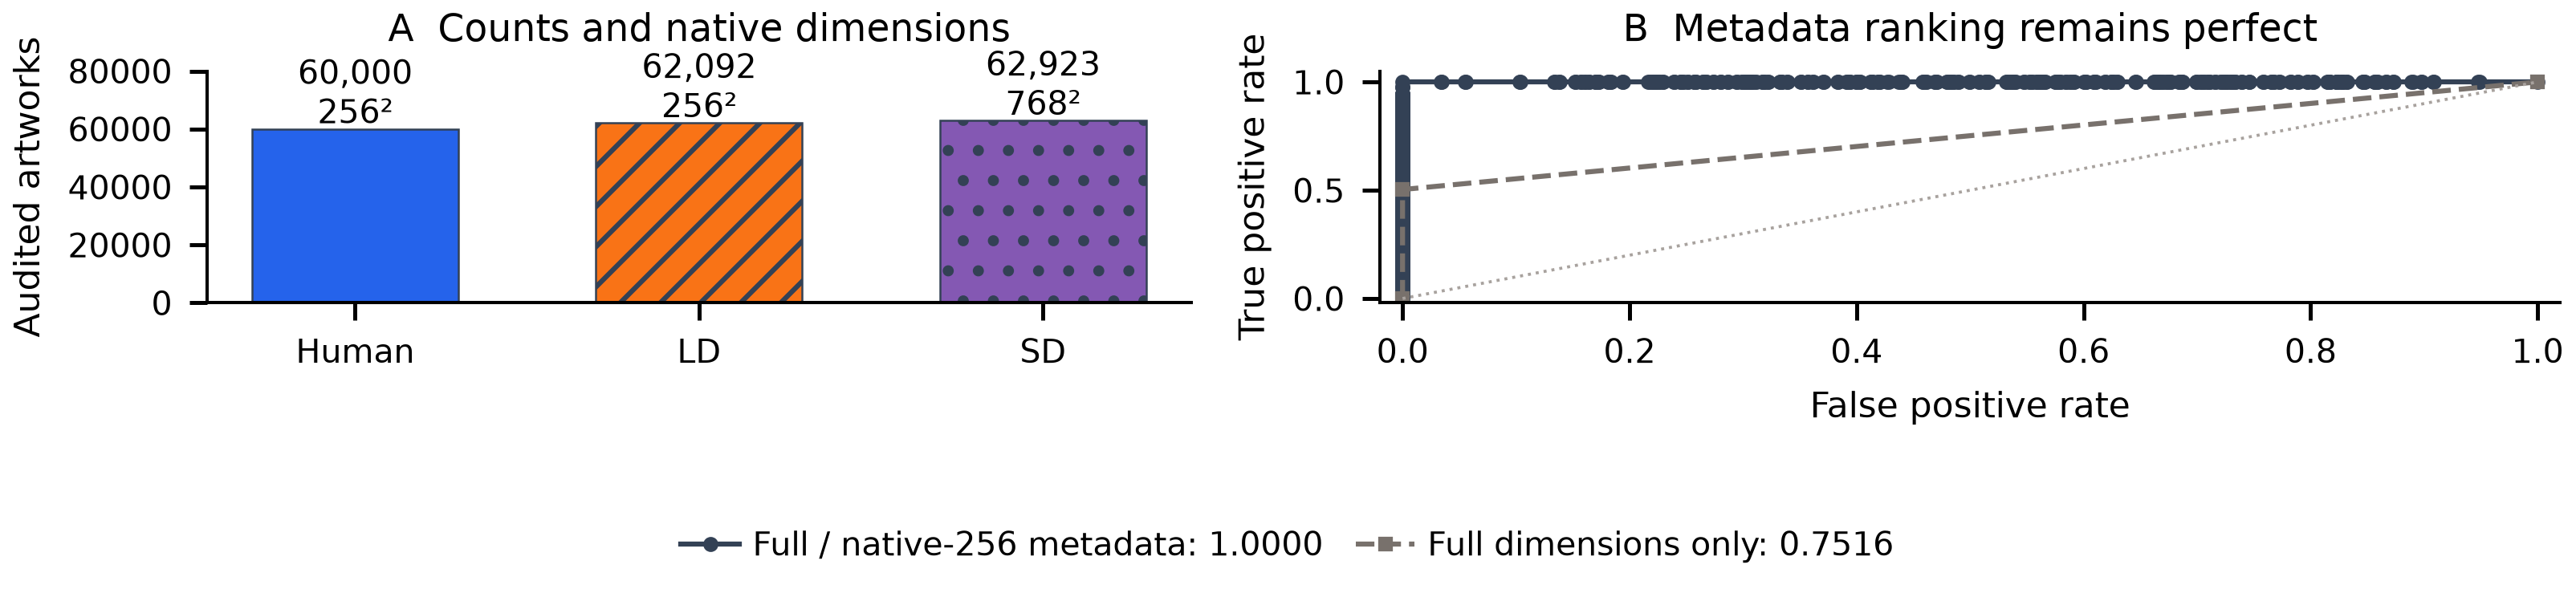
\includegraphics[width=\textwidth,height=1.65in,keepaspectratio]{figure_02.png}

\caption{All 185,015 files are audited; annotations show native dimensions. Full-release/native-256 metadata ROC curves coincide and are drawn once. Size matching leaves perfect technical label ranking, without proving use of that association by pixel probes.}\label{fig:f2}

\end{figure*}

\subsection{Baselines, Metrics and Computing Environment}
Five logistic probes use identical 6,000 test IDs: Handcrafted (104-D), FFT-only (36-D), Metadata-only (the implementation's \texttt{metadata\_gated} probe), frozen ResNet-50 \cite{resnet} 2,048-D and frozen DINOv2 \cite{dinov2} ViT-S/14 384-D. ResNet-50 uses ImageNet \cite{imagenet} weights IMAGENET1K\_V2 from torchvision \cite{torchvision}. Encoder views are resized to 224 pixels and ImageNet normalized; four float32 embeddings are averaged after CUDA FP16 inference (32-quadrant batches, four loaders). The encoders are not fine-tuned. Metadata inputs are width, height, bytes, aspect ratio, subsampling, progressive flag and quantization-table mean. Median imputation and robust scaling use development only; deep embeddings use StandardScaler. $C_{\mathrm{solver}}\in\{0.001,0.01,0.1,1,10,100\}$ maximizes validation AUROC, and the positive threshold maximizes validation F1. Final fitting uses development only.

Fifteen-bin expected calibration error (ECE) measures calibration. Origin silhouette \cite{silhouette} is $(b-a)/\max(a,b)$ for mean same-origin distance $a$ and other-origin distance $b$; unlabeled $k=2$ adjusted Rand index (ARI) compares clusters with origin after fitting. On a fixed 3,000-artwork subset, trustworthiness $T(15)$ \cite{venna} penalizes false neighbors and continuity $C(15)$ lost neighbors. This continuity is distinct from complexity and regularization; threshold/macro metrics are defined in Table~\ref{tab:essential}.

The recorded environment uses Python 3.12.16, NumPy 2.5.4 \cite{numpy}, SciPy 1.18.1 \cite{scipy}, scikit-learn 1.9.1, pandas 3.1.1, PyTorch 2.6.0+cu124 \cite{pytorch}, torchvision 0.21.0+cu124, Streamlit 1.67.0 and Plotly 7.1.0. Hardware is a GTX 1650 SUPER (4 GB), 16 GB RAM and 12 logical CPUs. Appendix A records driver/cuDNN, solver/projection settings and stage timings. Synthetic tests cover feature invariants and numerical routines, not attribution validity.

Relative to the preceding report, aggregate probe intervals, paired differences, five grouped repartitions, mixed-cohort F1 and JPEG quantization means are additional manuscript summaries from the same cached features, predictions and metadata; no new data were collected. Released scripts and CSVs identify their provenance.

\section{Results and Analysis}
\subsection{Held-Out Probe Evaluation}
Tables~\ref{tab:t4}--\ref{tab:seeds} and Fig.~\ref{fig:f3} compare the same primary test identities. ResNet-50 (0.9999) and DINOv2 (0.9997) outperform handcrafted AUROC 0.9824. Metadata-only achieves AUROC 1.0000, yet ECE 0.1940 shows that perfect ranking need not imply calibration. Full standardized/PCA unlabeled ARI remains near zero (maximum 0.0034): supervised ranking need not reveal natural origin clusters.
\begin{table*}[t]
\caption{Primary-test metrics (6,000 artworks). Accuracy equals balanced accuracy (BA); precision/recall/F1 use diffusion-positive labels. Macro scores average ten styles. Percentile 95\% intervals use 1,000 origin-stratified source-group draws with fits/thresholds fixed. Selected settings appear in Appendix A.}\label{tab:t4}\label{tab:essential}
\centering\footnotesize\setlength{\tabcolsep}{3pt}\renewcommand{\arraystretch}{1.10}
\begin{tabularx}{\textwidth}{>{\hsize=1.471\hsize\linewidth=\hsize\raggedright\arraybackslash}X>{\hsize=2.059\hsize\linewidth=\hsize\raggedright\arraybackslash}X>{\hsize=1.353\hsize\linewidth=\hsize\raggedright\arraybackslash}X>{\hsize=0.553\hsize\linewidth=\hsize\raggedright\arraybackslash}X>{\hsize=0.553\hsize\linewidth=\hsize\raggedright\arraybackslash}X>{\hsize=0.553\hsize\linewidth=\hsize\raggedright\arraybackslash}X>{\hsize=0.494\hsize\linewidth=\hsize\raggedright\arraybackslash}X>{\hsize=0.965\hsize\linewidth=\hsize\raggedright\arraybackslash}X}
\toprule
\textbf{Probe} & \textbf{AUROC [95\% CI]} & \textbf{F1 [95\% CI]} & \textbf{Acc./BA} & \textbf{Prec.} & \textbf{Recall} & \textbf{ECE} & \textbf{Macro AUC/F1}\\\midrule
{}Handcrafted (104-D) & 0.982415 [0.978332, 0.986003] & 0.9420 [0.9347, 0.9487] & 0.9407 & 0.9213 & 0.9637 & 0.0154 & 0.9817/0.9422\\
{}FFT-only (36-D) & 0.683901 [0.664844, 0.701442] & 0.6830 [0.6605, 0.7027] & 0.5960 & 0.5620 & 0.8703 & 0.0500 & 0.6909/0.6826\\
{}Metadata-only & 1.000000 [1.000000, 1.000000] & 0.9997 [0.9992, 1.0000] & 0.9997 & 1.0000 & 0.9993 & 0.1940 & 1.0000/0.9997\\
{}ResNet-50 (frozen) & 0.999945 [0.999868, 0.999988] & 0.9972 [0.9957, 0.9985] & 0.9972 & 0.9973 & 0.9970 & 0.0022 & 0.9999/0.9972\\
{}DINOv2 (frozen) & 0.999688 [0.999296, 0.999939] & 0.9955 [0.9936, 0.9973] & 0.9955 & 0.9947 & 0.9963 & 0.0021 & 0.9997/0.9955\\
\bottomrule\end{tabularx}
\end{table*}

Paired intervals in Table~\ref{tab:paired} use identical origin-stratified group draws and concern predictive ranking, not attribution. Table~\ref{tab:seeds} repartitions the same cohort at seeds 43--47 and refits preprocessing, regularization and thresholds. Cached embeddings and original seed-42 extraction calibration remain fixed; these are conditional split sensitivities, not full pipeline replications.
\begin{table}[t]\caption{Paired AUROC differences, handcrafted minus comparator. 95\% percentile source-group intervals condition on frozen fits.}\label{tab:paired}\centering\footnotesize\begin{tabular}{lrr}\toprule
\textbf{Comparator} & \textbf{Difference} & \textbf{95\% CI}\\\midrule
{}FFT-only (36-D) & 0.2985 & [+0.2812, +0.3176]\\
{}ResNet-50 (frozen) & -0.0175 & [-0.0216, -0.0140]\\
{}DINOv2 (frozen) & -0.0173 & [-0.0213, -0.0138]\\
\bottomrule\end{tabular}\end{table}
\begin{table}[t]\caption{Five grouped repartitions of the same frozen cohort, seeds 43--47. Mean $\pm$ sample SD; not independent data collections.}\label{tab:seeds}\centering\footnotesize\begin{tabular}{lcc}\toprule
\textbf{Probe} & \textbf{AUROC} & \textbf{F1}\\\midrule
{}DINOv2 (frozen) & 0.999838 ± 0.000019 & 0.9957 ± 0.0006\\
{}FFT-only (36-D) & 0.688800 ± 0.008013 & 0.6801 ± 0.0042\\
{}Handcrafted (104-D) & 0.981684 ± 0.002027 & 0.9397 ± 0.0041\\
{}Metadata-only & 1.000000 ± 0.000000 & 0.9997 ± 0.0003\\
{}ResNet-50 (frozen) & 0.999871 ± 0.000024 & 0.9954 ± 0.0013\\
\bottomrule\end{tabular}\end{table}
\begin{figure*}[t]

\centering

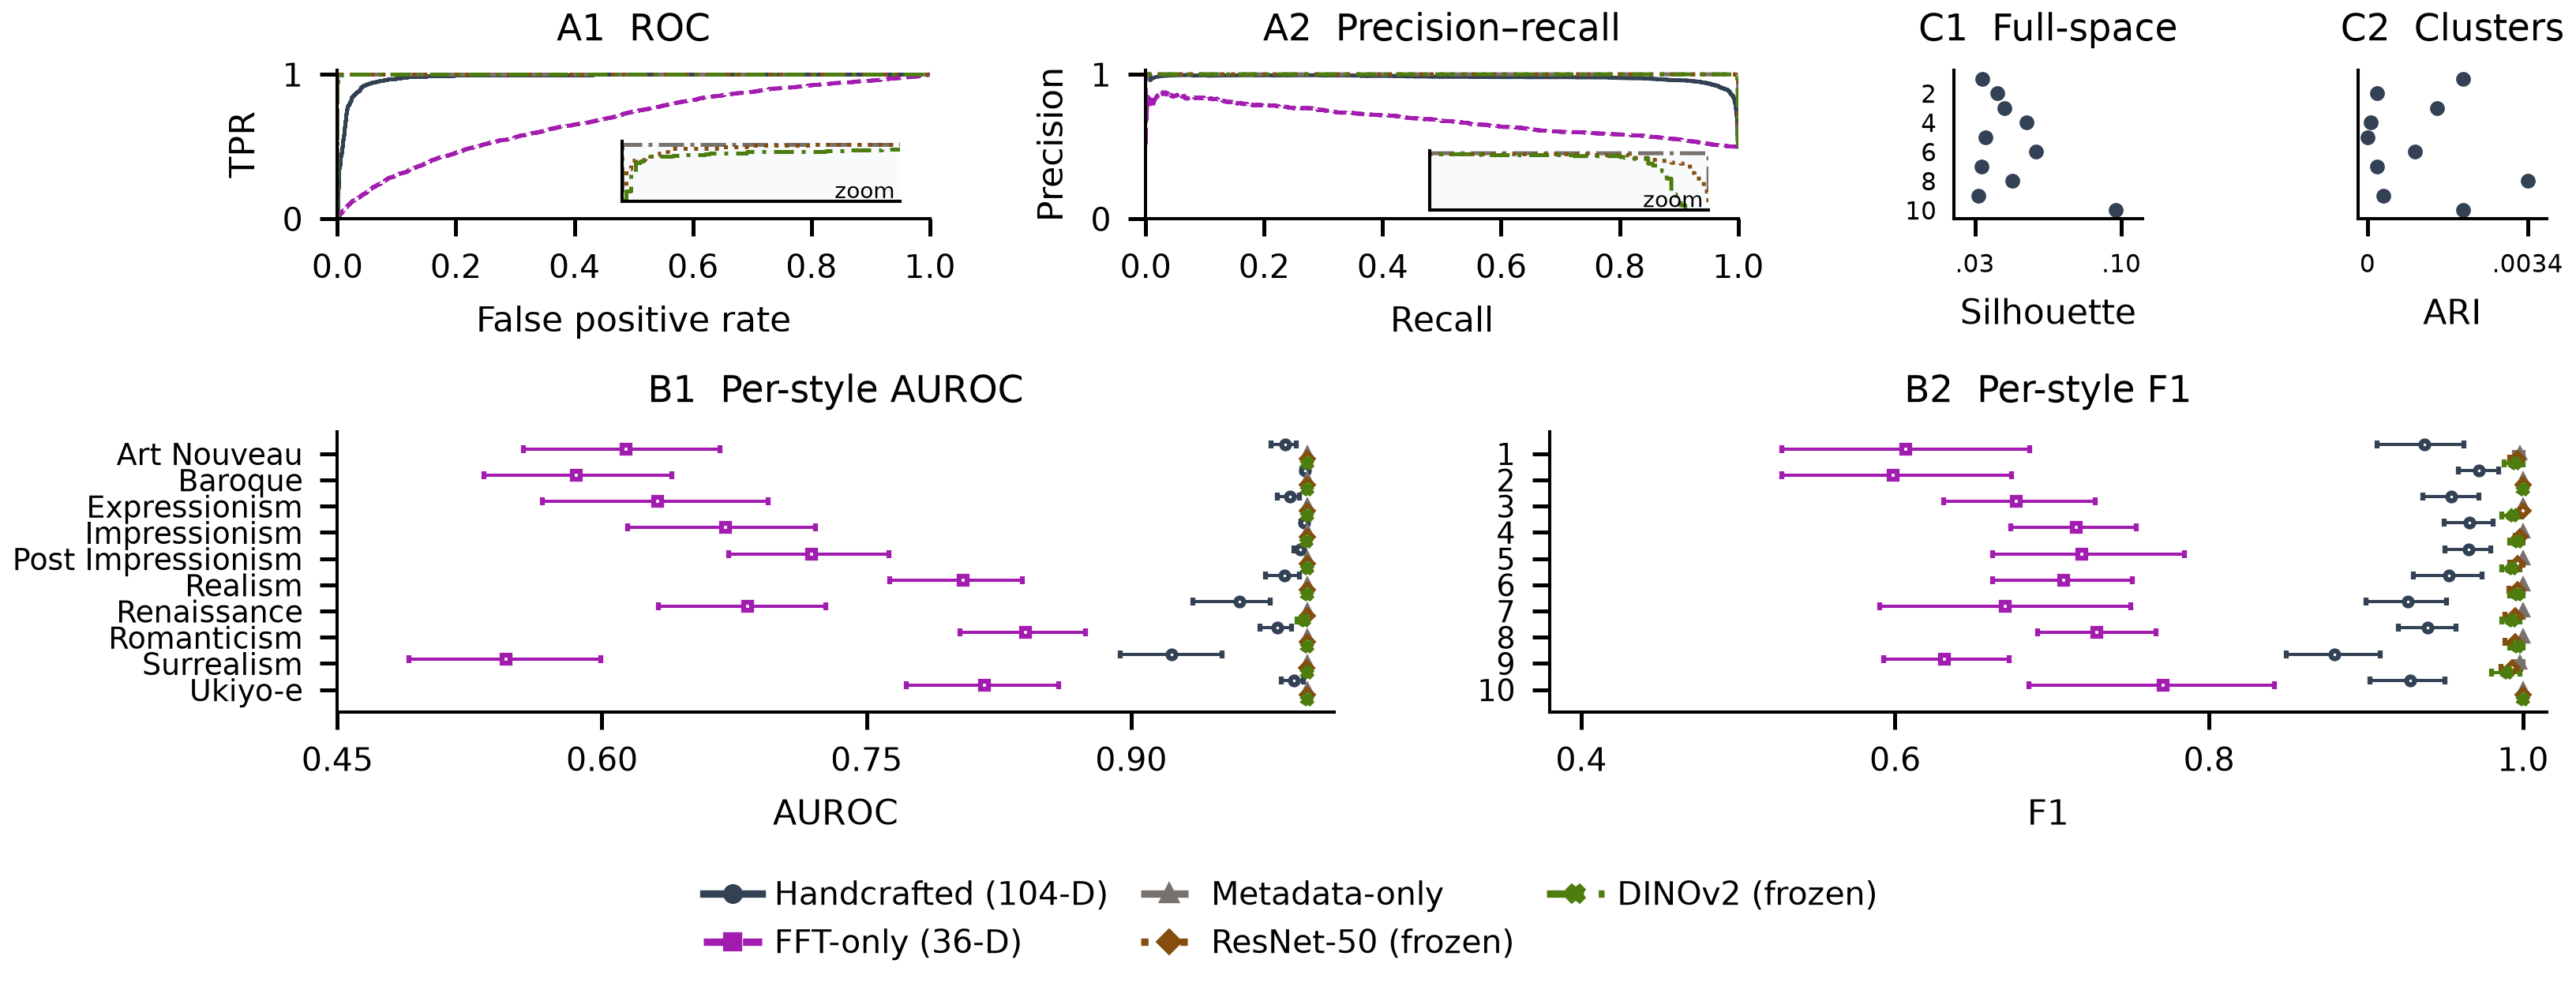
\includegraphics[width=\textwidth,height=2.8in,keepaspectratio]{figure_03.png}

\caption{Five probes share 6,000 test IDs; whiskers are frozen-fit group-bootstrap 95\% intervals. Insets zoom ROC to FPR 0--0.02/TPR 0.98--1 and PR to [0.98,1]². C1/C2 rows follow B1 top-to-bottom (alternating style keys shown); leader lines are omitted. Low ARI coexists with strong supervised ranking.}\label{fig:f3}

\end{figure*}

\subsection{Entropy--Complexity Atlas and Projection Fidelity}
Figure~\ref{fig:f4} compares shared-axis centroids and distributions. Most LD clouds have lower entropy and higher complexity than Human clouds, with heterogeneous descriptive magnitudes. Equal artwork counts do not imply equal source-group precision.
\begin{figure*}[t]

\centering

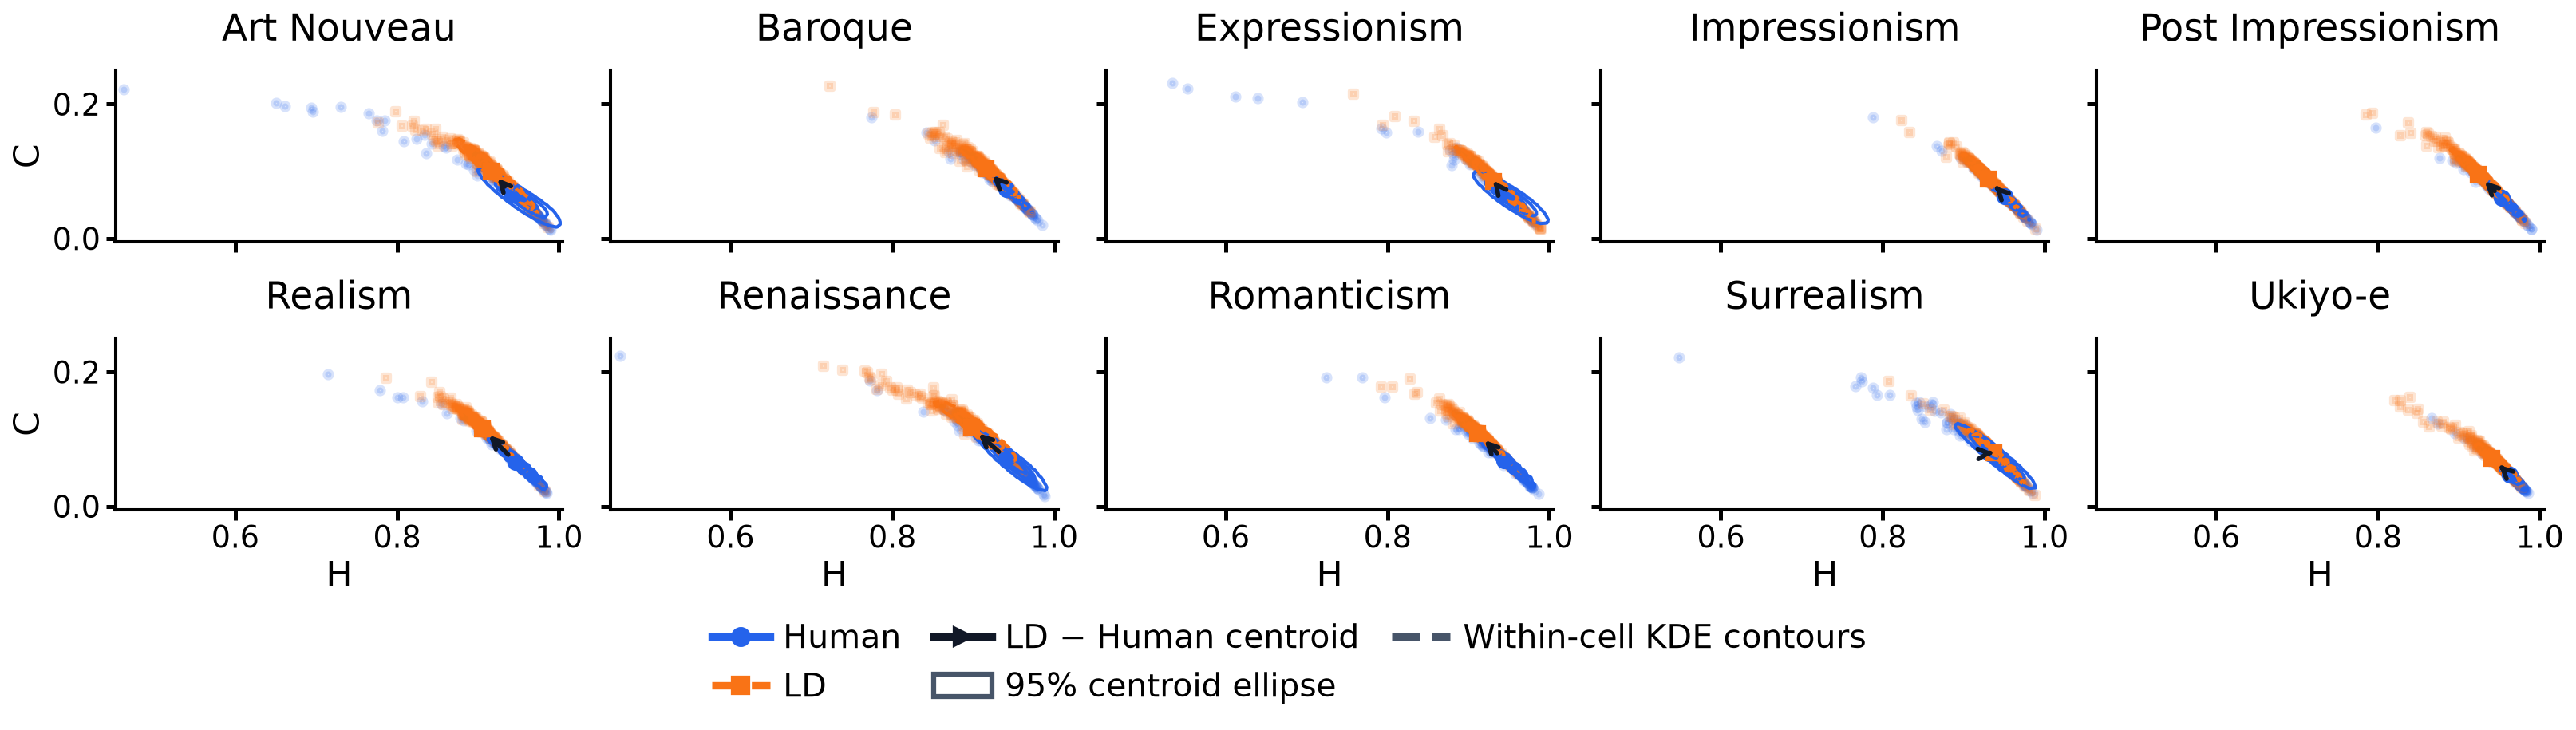
\includegraphics[width=\textwidth,height=2.05in,keepaspectratio]{figure_04.png}

\caption{Shared-axis H--C atlas (open Human circles, filled LD squares) with LD-minus-Human arrows, Gaussian 95\% centroid ellipses (500 group resamples) and within-cell KDE contours (15/40/70\% of peak). Full movement names reveal heterogeneous descriptive displacements, without establishing attribution.}\label{fig:f4}

\end{figure*}
PCA2 explains 93.57\% of development variance but attains $T(15)=0.6928$ and $C(15)=0.7571$; PCA3 reaches 0.7800/0.8869 (Table~\ref{tab:t5}). Fifteen t-SNE \cite{tsne} runs cover seeds 42--46 and perplexities 15/30/50, with trustworthiness 0.9101--0.9185. Figure~\ref{fig:f5} fixes perplexity 30/seed 42 without selecting test separation. Seed ranges measure algorithmic sensitivity; distance inference stays in standardized features or fixed PCA.
\begin{table}[tb]
\caption{Neighborhood fidelity on the fixed audit subset. t-SNE entries give min--max over five seeds, not confidence intervals.}\label{tab:t5}
\centering
\footnotesize
\setlength{\tabcolsep}{3pt}
\renewcommand{\arraystretch}{1.12}
\begin{tabularx}{\columnwidth}{>{\hsize=1.100\hsize\linewidth=\hsize\raggedright\arraybackslash}X>{\hsize=0.600\hsize\linewidth=\hsize\raggedright\arraybackslash}X>{\hsize=1.100\hsize\linewidth=\hsize\raggedright\arraybackslash}X>{\hsize=1.100\hsize\linewidth=\hsize\raggedright\arraybackslash}X>{\hsize=1.100\hsize\linewidth=\hsize\raggedright\arraybackslash}X}
\toprule
\textbf{Space} & \textbf{Seeds} & \textbf{T(15)} & \textbf{C(15)} & \textbf{Variance}\\\midrule
{}PCA 2D & fixed & 0.6928 & 0.7571 & 0.9357\\
{}PCA 3D & fixed & 0.7800 & 0.8869 & 0.9512\\
{}t-SNE p=15 & 42--46 & 0.9101--0.9118 & 0.9069--0.9071 & ---\\
{}t-SNE p=30 & 42--46 & 0.9148--0.9162 & 0.9119--0.9132 & ---\\
{}t-SNE p=50 & 42--46 & 0.9165--0.9185 & 0.9140--0.9156 & ---\\
\bottomrule\end{tabularx}
\end{table}
\begin{figure*}[t]

\centering

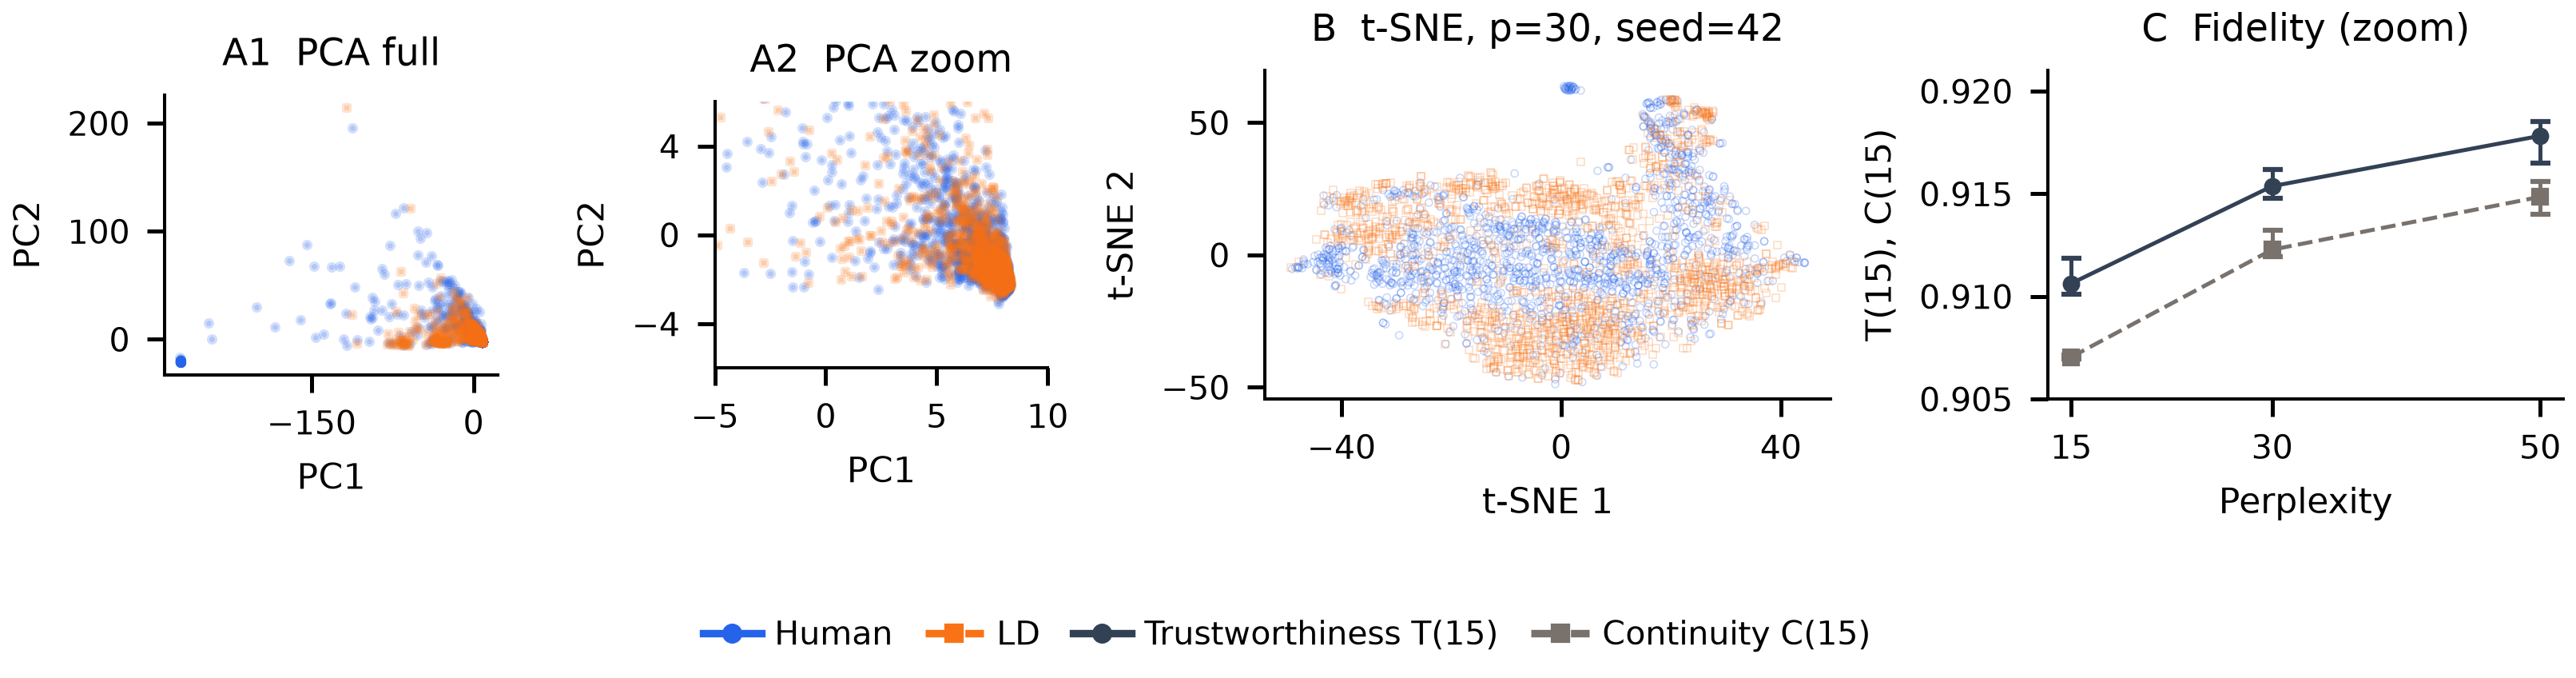
\includegraphics[width=\textwidth,height=1.9in,keepaspectratio]{figure_05.png}

\caption{Equal-aspect PCA retains all points (A1); A2 zooms PC1 to [$-$5,10] and PC2 to [$-$6,6]. Transparent t-SNE uses perplexity 30, seed 42. Fidelity axis 0.905--0.921 magnifies small differences; whiskers are seed ranges, not confidence intervals.}\label{fig:f5}

\end{figure*}

\subsection{Spectral, Wavelet and Within-Style Contrasts}
Figure~\ref{fig:f6} contrasts radial power shares and raw-luminance Haar energy. Human and LD spectra are broadly similar, while wavelet bands and style-specific features differ. SD remains a resized sensitivity. Figure~\ref{fig:f7} and Table~\ref{tab:t6} summarize mean standardized $W_1$ and mean signed shifts by family. Averaging signed constituents can cancel opposing directions; family means are not independent tests. Every family contains an exploratory constituent pass; redundant asterisks are omitted, and no family-level test or confirmation is implied.
\begin{figure*}[t]

\centering

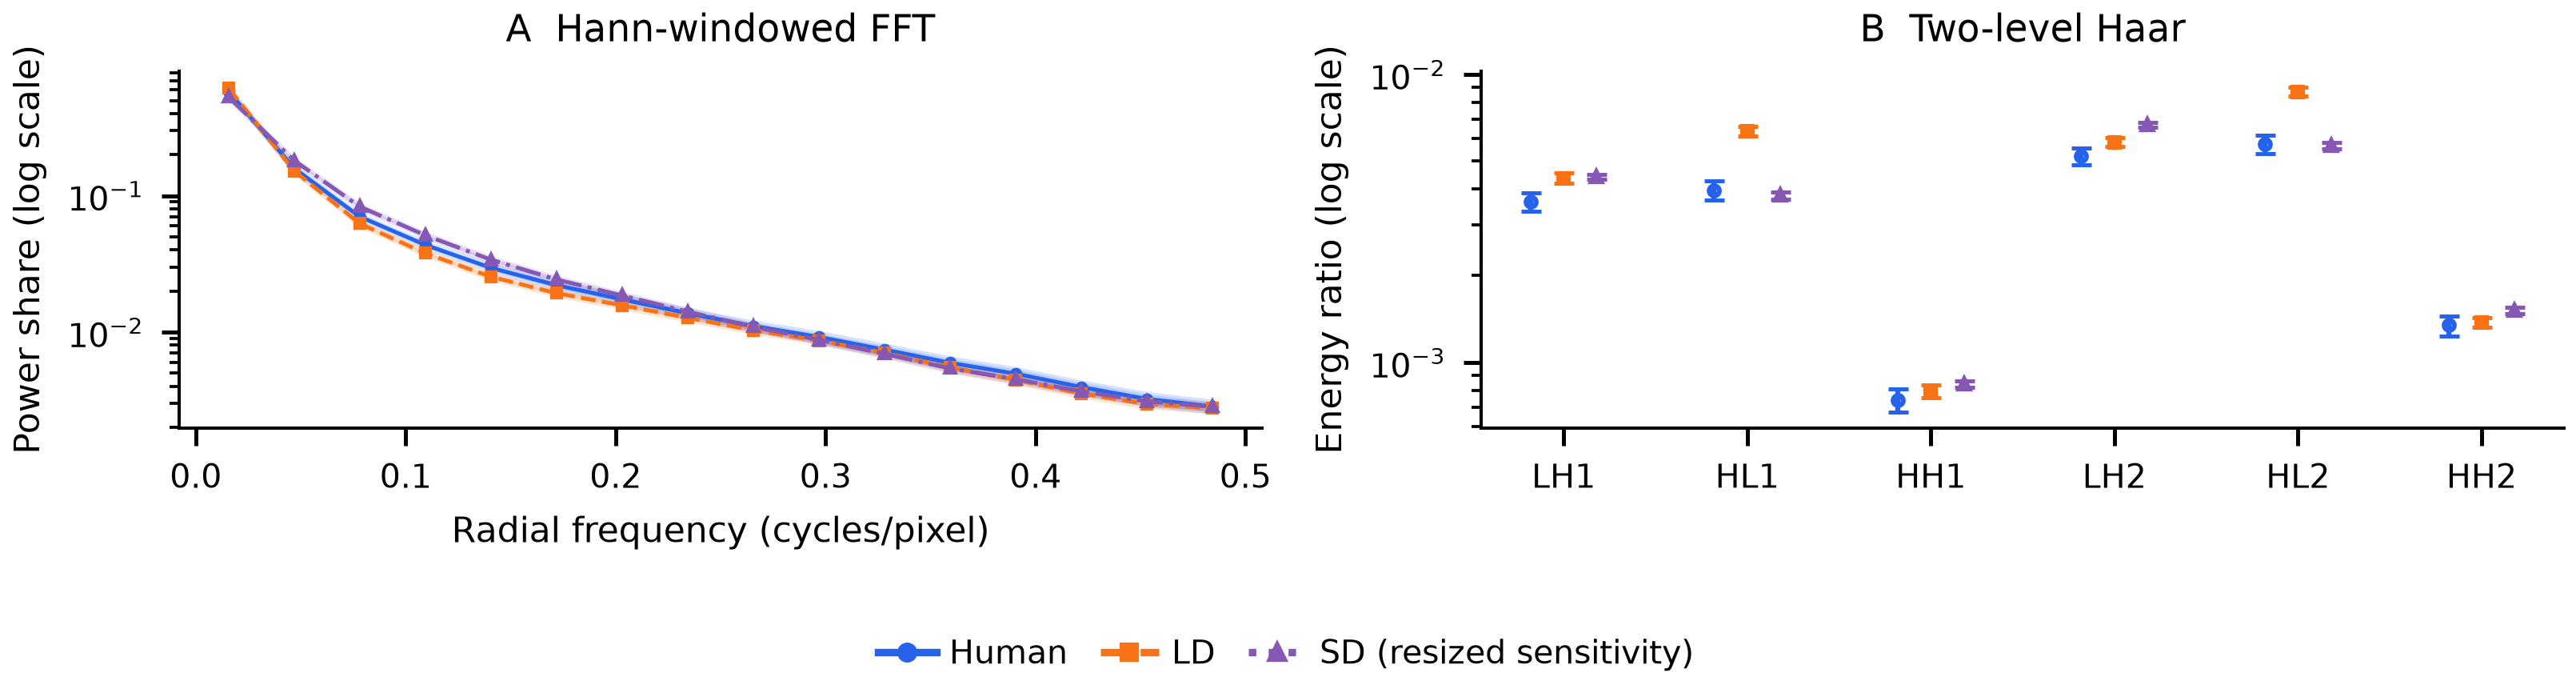
\includegraphics[width=\textwidth,height=1.95in,keepaspectratio]{figure_06.png}

\caption{FFT/Haar means with 1,000-group-bootstrap 95\% intervals. Small open Haar markers expose whiskers; LL2 remains in normalization. SD resizing is descriptive. Broadly similar spectra do not eliminate style-specific differences.}\label{fig:f6}

\end{figure*}
\begin{figure*}[t]

\centering

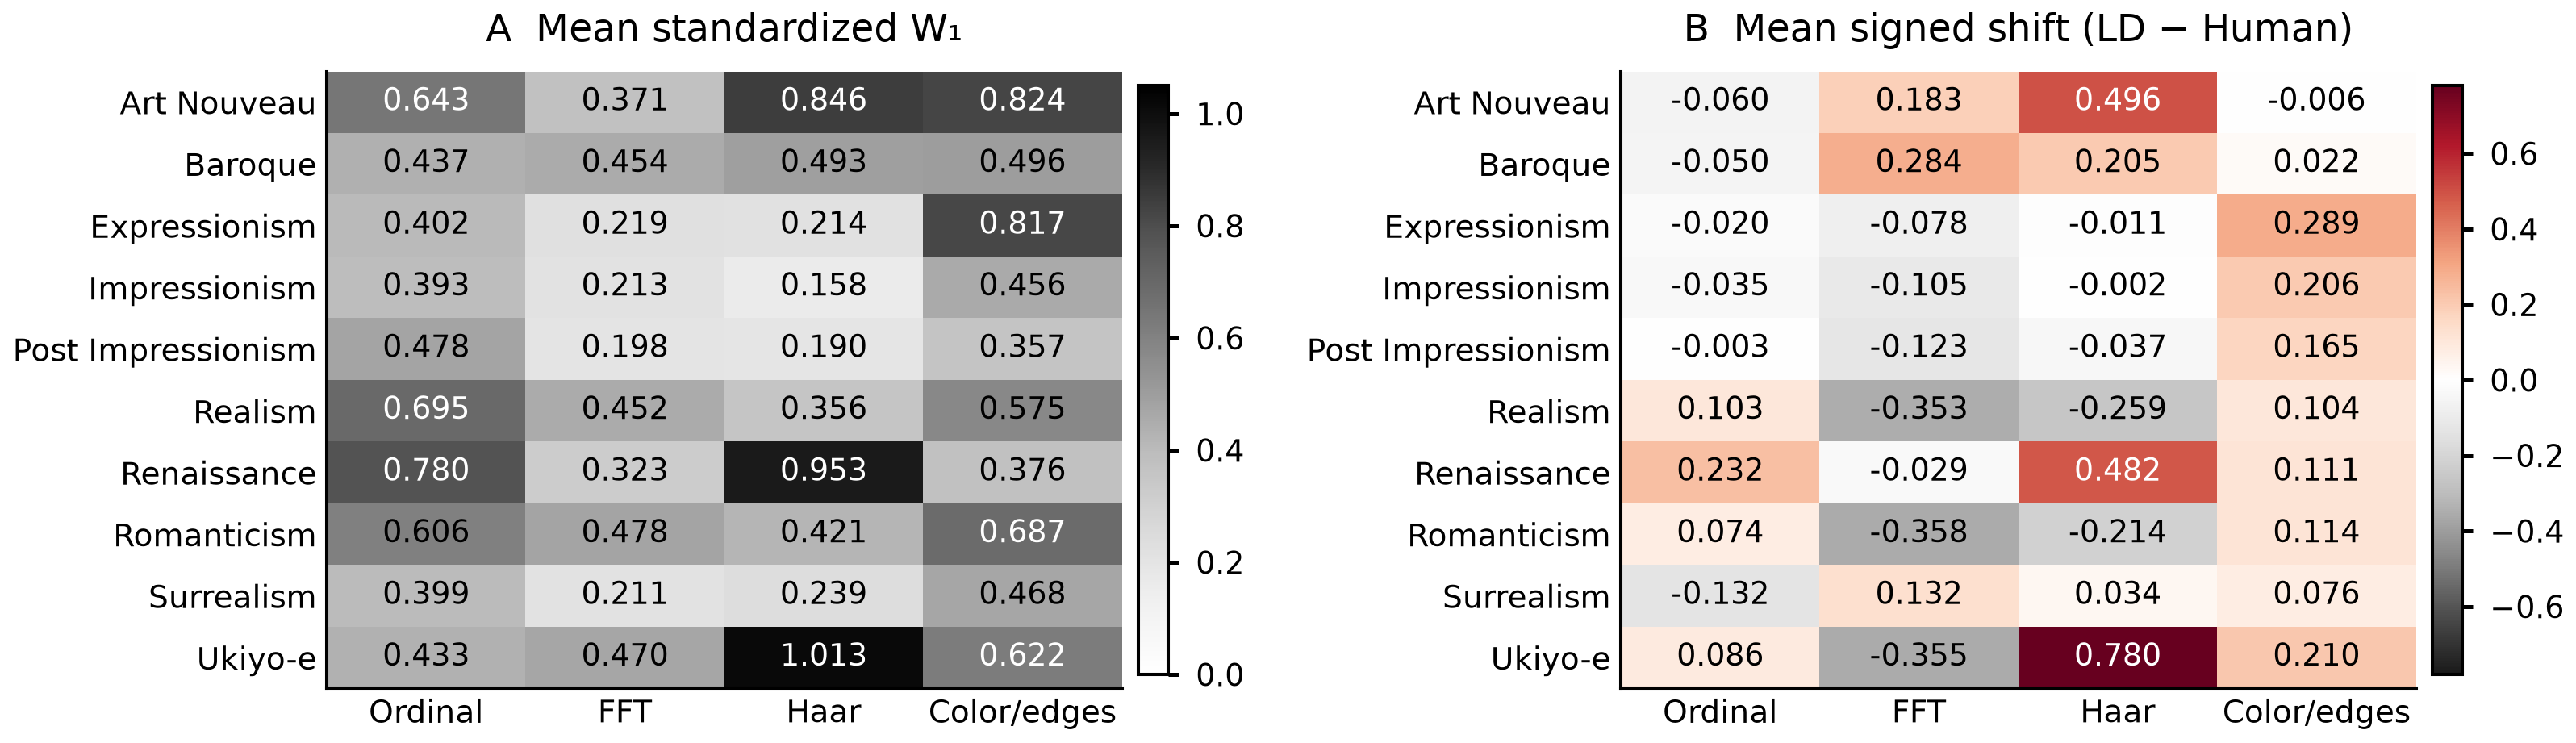
\includegraphics[width=\textwidth,height=2.05in,keepaspectratio]{figure_07.png}

\caption{Family-average W$_1$ and signed median shifts. All families contain exploratory constituents; redundant asterisks are omitted. The W$_1$ scale ends at 1.05 (including 1.013); teal/ochre signed colors are zero-centered. These shifts remain unconfirmed.}\label{fig:f7}

\end{figure*}
\begin{table*}[tb]
\caption{Ten-style family summaries: mean standardized W1 / mean signed shift; last column counts constituent exploratory passes.}\label{tab:t6}
\centering
\footnotesize
\setlength{\tabcolsep}{3pt}
\renewcommand{\arraystretch}{1.12}
\begin{tabularx}{\textwidth}{>{\hsize=1.320\hsize\linewidth=\hsize\raggedright\arraybackslash}X>{\hsize=1.020\hsize\linewidth=\hsize\raggedright\arraybackslash}X>{\hsize=1.020\hsize\linewidth=\hsize\raggedright\arraybackslash}X>{\hsize=1.020\hsize\linewidth=\hsize\raggedright\arraybackslash}X>{\hsize=1.020\hsize\linewidth=\hsize\raggedright\arraybackslash}X>{\hsize=0.600\hsize\linewidth=\hsize\raggedright\arraybackslash}X}
\toprule
\textbf{Style} & \textbf{Ordinal} & \textbf{FFT} & \textbf{Haar} & \textbf{Color / edges} & \textbf{Raw passes}\\\midrule
{}Art Nouveau & 0.643 / -0.060 & 0.371 / +0.183 & 0.846 / +0.496 & 0.824 / -0.006 & 58\\
{}Baroque & 0.437 / -0.050 & 0.454 / +0.284 & 0.493 / +0.205 & 0.496 / +0.022 & 68\\
{}Expressionism & 0.402 / -0.020 & 0.219 / -0.078 & 0.214 / -0.011 & 0.817 / +0.289 & 45\\
{}Impressionism & 0.393 / -0.035 & 0.213 / -0.105 & 0.158 / -0.002 & 0.456 / +0.206 & 55\\
{}Post-impr. & 0.478 / -0.003 & 0.198 / -0.123 & 0.190 / -0.037 & 0.357 / +0.165 & 37\\
{}Realism & 0.695 / +0.103 & 0.452 / -0.353 & 0.356 / -0.259 & 0.575 / +0.104 & 75\\
{}Renaissance & 0.780 / +0.232 & 0.323 / -0.029 & 0.953 / +0.482 & 0.376 / +0.111 & 33\\
{}Romanticism & 0.606 / +0.074 & 0.478 / -0.358 & 0.421 / -0.214 & 0.687 / +0.114 & 73\\
{}Surrealism & 0.399 / -0.132 & 0.211 / +0.132 & 0.239 / +0.034 & 0.468 / +0.076 & 48\\
{}Ukiyo-E & 0.433 / +0.086 & 0.470 / -0.355 & 1.013 / +0.780 & 0.622 / +0.210 & 50\\
\bottomrule\end{tabularx}
\end{table*}
The 542 exploratory passes among 1,040 tests cannot be confirmed because the common-support gate (Algorithm~\ref{alg:pipeline}, line 8) lacks verified subjects and encoding overlap. Adjusted probabilities cannot remove systematic bias. Supplementary Fig. S1, file \texttt{supplementary.pdf}, supplies the six development-selected feature rainclouds/ECDFs; selection does not use held-out effect strength.


\subsection{Interactive Visual Analytics}
\begin{figure*}[t]
\centering
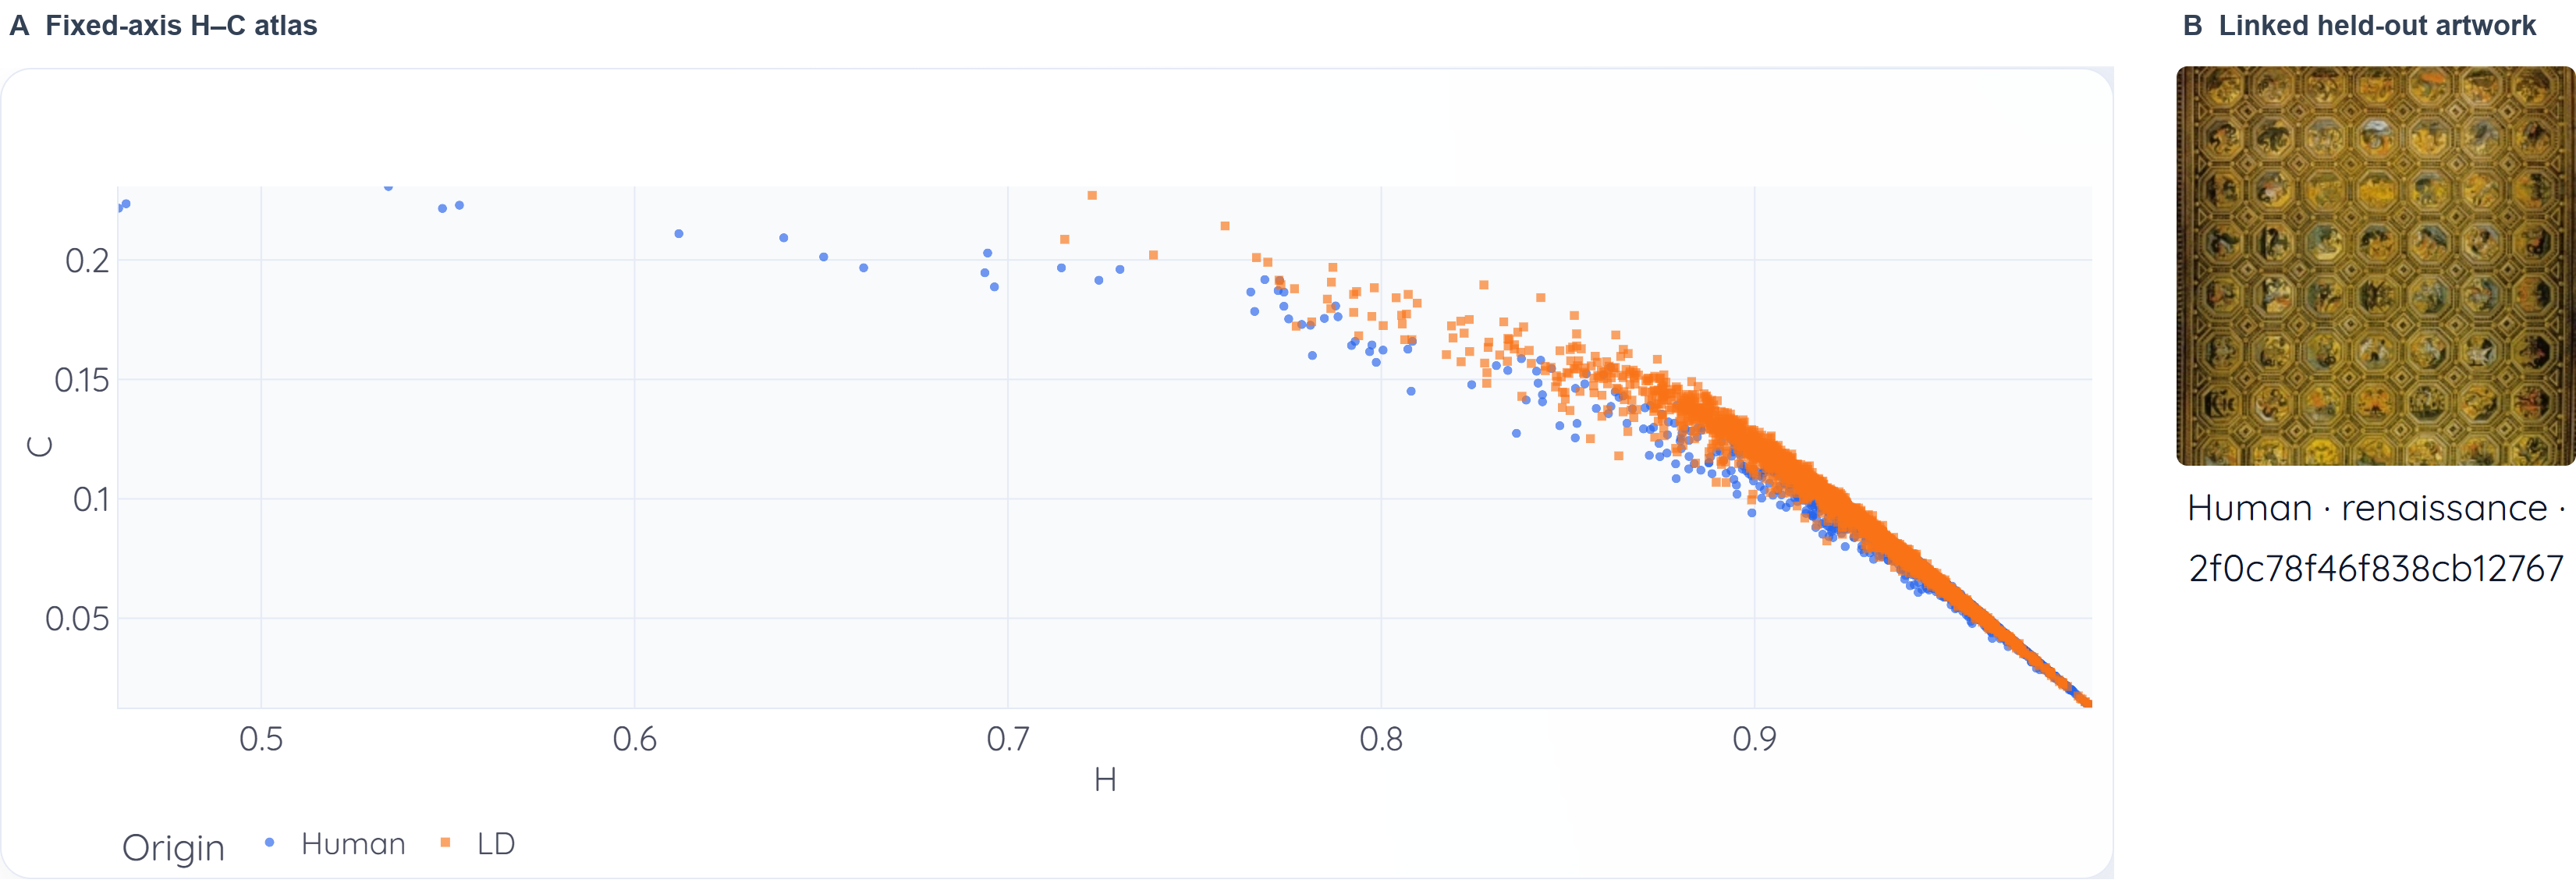
\includegraphics[width=\textwidth,height=1.65in,keepaspectratio]{figure_09.png}
\caption{Cropped dashboard atlas with H/C labels and a two-origin legend, linked to an actual held-out case. Movement identity remains in filters/hover; inspection does not establish attribution.}\label{fig:f9}
\end{figure*}

The Streamlit\footnote{\url{https://streamlit.io/}}/Plotly\footnote{\url{https://plotly.com/python/}} application links overview, atlas, manifold, spectra, drift and gallery views. Movement/origin filters and point selection link raw/hexagonal views to quadrants, FFT, Haar and color summaries. Axes stay fixed; density colors explicitly rescale to active counts. Figure~\ref{fig:f9} shows the linked interface; gate warnings persist. The compact dashboard retains all points but only eight pixel-inspectable cases; full drill-down requires local data/caches. No user-study gain is established.


\section{Comparison with Base Papers and State-of-the-Art}
\subsection{Base-Paper Summary}
The base papers are ArtBrain \cite{p1}, Kim et al. \cite{p2}, B-Free \cite{p3}, SCADET \cite{p4}, SPAI \cite{p5}, FIRE \cite{p6}, VIB-Net \cite{p7}, CoDA \cite{p8}, FakeBench \cite{p12} and SIDWA \cite{p14} (Table~\ref{tab:t7}). The remaining Table~\ref{tab:t1} studies are related work rather than base methods. No base-paper method was reimplemented; FFT-only is the matched internal ablation comparator, limiting external comparisons to source-reported protocols.

\begin{table*}[t]
\caption{Ten benchmark, feature and control bases, with published years. Manuscript versions follow Table I; starred results are source-reported.}\label{tab:t7}
\centering\fontsize{7.5}{8.6}\selectfont
\setlength{\tabcolsep}{3pt}\renewcommand{\arraystretch}{1.10}
\begin{tabularx}{\textwidth}{>{\hsize=0.824\hsize\linewidth=\hsize\raggedright\arraybackslash}X>{\hsize=0.961\hsize\linewidth=\hsize\raggedright\arraybackslash}X>{\hsize=0.961\hsize\linewidth=\hsize\raggedright\arraybackslash}X>{\hsize=1.098\hsize\linewidth=\hsize\raggedright\arraybackslash}X>{\hsize=0.686\hsize\linewidth=\hsize\raggedright\arraybackslash}X>{\hsize=1.647\hsize\linewidth=\hsize\raggedright\arraybackslash}X>{\hsize=0.824\hsize\linewidth=\hsize\raggedright\arraybackslash}X}
\toprule
\textbf{Authors / year} & \textbf{Problem} & \textbf{Method} & \textbf{Dataset} & \textbf{Metric} & \textbf{Reported result*} & \textbf{Limitation}\\\midrule
{}\cite{p1} Silva et al., 2026$\dagger$ & Joint source/style classification and generator attribution & AttentionConvNeXt & AI-ArtBench, 185,015 images, 10 styles & F1; attribution accuracy & Joint source/style F1 0.869; attribution accuracy 0.999; 60,000 Human / 125,015 generated & Joint task, different protocol\\
{}\cite{p2} Kim et al., 2025 & Observational style analysis in entropy-complexity space & Ordinal H-C & DeviantArt and Behance 2010--2020 & H and C; similarity relationships & 149,780 platform artworks; no matched Human--diffusion test & Platform art; no matched origin test\\
{}\cite{p3} Guillaro et al., 2025 & Bias-controlled general AI-image detection & Content-aligned DINOv2 & MS-COCO and self-conditioned synthetic images & Dataset counts; AUC; balanced accuracy & Training: 51,517 real / 309,102 generated images & Photographs, end-to-end training\\
{}\cite{p4} Zhang et al., 2025 & Full-image and local-image AI-art detection & Contrastive spectral attention & AI-ArtBench & ROC-AUC; accuracy & Full/local AUC 0.962/0.801; cross-model mean accuracy 0.81 & Different split/crop/model\\
{}\cite{p5} Karageorgiou et al., 2025 & AI-image detection & Spectral self-supervision & 13 generators; mixed real-image sources & ROC-AUC & Absolute AUC gain 5.5 percentage points across 13 generators & Cross-generator learned detector\\
{}\cite{p6} Chu et al., 2025 & Diffusion-image detection & Reconstruction error & DiffusionForensics and updated-generator benchmark & AUC; accuracy & Kandinsky3-trained (Table 2): mean AUC FIRE 78.1\% / FakeInversion 70.5\% & Source-specific trained detector\\
{}\cite{p7} Zhang et al., 2025 & Universal AI-image detection & Variational bottleneck & 15 generator columns in Table 1; 17 generators overall & Average precision & Table 1 mean AP: VIB-Net 95.53\% / NPR 89.98\% & AP, not AUROC\\
{}\cite{p8} Jia et al., 2026 & Cross-domain AI-image detection & Color probing & FakeForm, 62 domains & Accuracy; AP & FakeForm mean accuracy/AP 77.7\%/88.1\% & AP/domain endpoint differs\\
{}\cite{p12} Li et al., 2025$\dagger$ & Explainable image authenticity assessment & Multimodal explanations & FakeBench & Detection accuracy & Human overall average accuracy 74.51\% & Human/LMM endpoints\\
{}\cite{p14} Li et al., 2026 & Synthetic-image detection & Wavelet attention & SIDset; additional GenImage experiments & Accuracy; inference latency & Abstract: average accuracy >95\%; 18.2 ms on NVIDIA A100 & SIDset, different protocol\\
\bottomrule\end{tabularx}
\end{table*}
\subsection{Quantitative Side-by-Side Evaluation}
Table~\ref{tab:t8} distinguishes executed probes from starred source-reported scores. The mixed-cohort 9,000-image test yields AUROC 0.9220/F1 0.8977; its different class/source composition cannot isolate resolution effects. Incompatible endpoints retain their original metric labels.
\begin{table*}[t]
\caption{Comparable metric columns with protocol limits. Unstarred rows are executed probes; starred rows are original-paper AUROCs, not reproduced or matched evaluations.}\label{tab:t8}
\centering\footnotesize
\setlength{\tabcolsep}{3pt}\renewcommand{\arraystretch}{1.10}
\begin{tabularx}{\textwidth}{>{\hsize=0.964\hsize\linewidth=\hsize\raggedright\arraybackslash}X>{\hsize=1.446\hsize\linewidth=\hsize\raggedright\arraybackslash}X>{\hsize=0.542\hsize\linewidth=\hsize\raggedright\arraybackslash}X>{\hsize=0.542\hsize\linewidth=\hsize\raggedright\arraybackslash}X>{\hsize=1.506\hsize\linewidth=\hsize\raggedright\arraybackslash}X}
\toprule
\textbf{Method} & \textbf{Protocol / test} & \textbf{AUROC} & \textbf{F1} & \textbf{Scope}\\\midrule
{}Handcrafted (104-D) & Primary / 6,000 & 0.9824 & 0.9420 & Implemented logistic probe\\
{}FFT-only (36-D) & Primary / 6,000 & 0.6839 & 0.6830 & Implemented logistic probe\\
{}Metadata-only & Primary / 6,000 & 1.0000 & 0.9997 & Implemented logistic probe\\
{}ResNet-50 (frozen) & Primary / 6,000 & 0.9999 & 0.9972 & Implemented logistic probe\\
{}DINOv2 (frozen) & Primary / 6,000 & 0.9997 & 0.9955 & Implemented logistic probe\\
{}Unmatched mixed & Human vs. LD+SD / 9,000 & 0.9220 & 0.8977 & Different source mixture\\
{}SCADET full* & AI-ArtBench / 7:1:2 & 0.9620 & --- & Different model/split\\
{}SCADET local* & AI-ArtBench / 7:1:2 & 0.8010 & --- & Different crop protocol\\
{}B-Free* & Aligned photographs & 0.9900 & --- & BA 0.952*; end-to-end\\
{}SPAI* & 13 generators & 0.9100 & --- & Reported mean AUC\\
\bottomrule\end{tabularx}
\end{table*}
\subsection{Methodological Differences}
ArtBrain supplies the release and learned joint tasks, whereas the present binary probe isolates native-resolution Human--LD ranking and explicitly audits encoding. Kim et al.'s observational entropy--complexity analysis motivates named coordinates; neither its art-platform study nor the present atlas establishes an origin intervention.

SCADET and SPAI train spectral representations; FIRE learns reconstruction evidence. The present fixed FFT/Haar descriptors and family ablations expose measured contributions without reproducing those networks. B-Free controls photographic content during training, while the present subject audit cannot establish such alignment. Its value is identifying this missing support rather than claiming equivalent robustness.

VIB-Net targets generalization with a learned bottleneck, CoDA probes color-domain shifts, and SIDWA learns wavelet attention. The proposed frozen/linear evaluation measures conditional prediction and transparent shifts, without unseen-generator evidence. FakeBench evaluates multimodal explanations; the artwork-linked gallery provides pixel/feature traces but no verified semantic grounding or user-study equivalence. 

\subsection{Absolute and Relative Differences}
The handcrafted-minus-ResNet-50 AUROC difference is -0.0175 (-1.75\%; 95\% interval $[-0.0216,-0.0140]$), and the handcrafted-minus-DINOv2 difference is -0.0173 (-1.73\%). Relative differences divide the unrounded score difference by the comparator's AUROC. Against FFT-only, the internal ablation comparator, the gain is +0.2985 AUROC (+43.65\%) and +0.2590 F1 (+37.93\%); each denominator is the corresponding FFT-only score.

Ordinal removal produces the largest family loss (Table~\ref{tab:t9}), supporting predictive complementarity rather than causal allocation. Cross-protocol AUROC differences are SCADET local: +0.1814 (+22.65\%); SCADET full: +0.0204 (+2.12\%); SPAI mean: +0.0724 (+7.96\%); B-Free: -0.0076 (-0.77\%). Each percentage uses the corresponding paper-reported score as denominator; none is a verified reproduced-method gain. No delta is computed for incompatible F1, AP, accuracy or human/LMM tasks.

\subsection{Fairness and Limitations}
SCADET uses 7:1:2 rather than grouped 60:20:20 splitting and includes resized native-$768^2$ SD; equivalent source-group protection is unverified. ArtBrain's joint F1 0.869*/attribution accuracy 0.999* use different targets, and its training description reuses test as validation. B-Free's 99.0\%* AUROC uses end-to-end content-aligned photographic training, not frozen artwork probing. These differences preclude a matched external leaderboard.

\section{Ablation Study and Perturbation Robustness}
\subsection{Feature Families, Color and Geometry}
Thirteen paired variants in Table~\ref{tab:t9} and Fig.~\ref{fig:f10} refit preprocessing/probes on development and retain held-out IDs. Removing ordinal features causes the largest family loss, $-0.0744$ AUROC (interval in Table~\ref{tab:t9}), followed by color/edges ($-0.0248$), FFT ($-0.0111$) and Haar ($-0.0035$). Ordinal-only attains AUROC 0.8888 and the largest origin-silhouette increase, $+0.0955$. Greater silhouette does not establish robustness or attribution.
\begin{table*}[t]
\caption{Thirteen paired ablations. Dim. is predictor dimensionality; $\Delta$ silhouette is variant minus baseline. Intervals refer to AUROC differences; silhouette uncertainty conditions on cached geometry.}\label{tab:t9}
\centering\footnotesize
\setlength{\tabcolsep}{3pt}\renewcommand{\arraystretch}{1.10}
\begin{tabularx}{\textwidth}{>{\hsize=1.842\hsize\linewidth=\hsize\raggedright\arraybackslash}X>{\hsize=0.368\hsize\linewidth=\hsize\raggedright\arraybackslash}X>{\hsize=0.737\hsize\linewidth=\hsize\raggedright\arraybackslash}X>{\hsize=0.737\hsize\linewidth=\hsize\raggedright\arraybackslash}X>{\hsize=0.737\hsize\linewidth=\hsize\raggedright\arraybackslash}X>{\hsize=1.842\hsize\linewidth=\hsize\raggedright\arraybackslash}X>{\hsize=0.737\hsize\linewidth=\hsize\raggedright\arraybackslash}X}
\toprule
\textbf{Variant} & \textbf{Dim.} & \textbf{AUROC} & \textbf{F1} & \textbf{$\Delta$AUC} & \textbf{95\% CI} & \textbf{$\Delta$ silhouette}\\\midrule
{}without Ordinal & 96 & 0.9080 & 0.8443 & -0.0744 & [-0.0842, -0.0654] & -0.0027\\
{}only Ordinal & 8 & 0.8888 & 0.8153 & -0.0936 & [-0.1045, -0.0836] & 0.0955\\
{}without FFT & 68 & 0.9713 & 0.9205 & -0.0111 & [-0.0142, -0.0082] & 0.0061\\
{}only FFT & 36 & 0.6839 & 0.6830 & -0.2985 & [-0.3176, -0.2812] & -0.0041\\
{}without Haar & 90 & 0.9789 & 0.9349 & -0.0035 & [-0.0048, -0.0021] & -0.0035\\
{}only Haar & 14 & 0.7659 & 0.7322 & -0.2165 & [-0.2334, -0.2017] & 0.0262\\
{}without Color/edges & 58 & 0.9576 & 0.9009 & -0.0248 & [-0.0303, -0.0201] & 0.0147\\
{}only Color/edges & 46 & 0.8672 & 0.8039 & -0.1152 & [-0.1286, -0.1016] & -0.0010\\
{}HSV & 86 & 0.9804 & 0.9398 & -0.0020 & [-0.0030, -0.0011] & -0.0020\\
{}Lab & 78 & 0.9791 & 0.9349 & -0.0033 & [-0.0053, -0.0017] & 0.0203\\
{}full 256 & 51 & 0.9790 & 0.9329 & -0.0034 & [-0.0058, -0.0014] & 0.0189\\
{}five 128 crops & 104 & 0.9810 & 0.9398 & -0.0014 & [-0.0028, +0.0000427] & -0.0043\\
{}ties excluded & 104 & 0.9753 & 0.9253 & -0.0072 & [-0.0091, -0.0053] & -0.0002\\
\bottomrule\end{tabularx}
\end{table*}
\begin{figure*}[t]

\centering

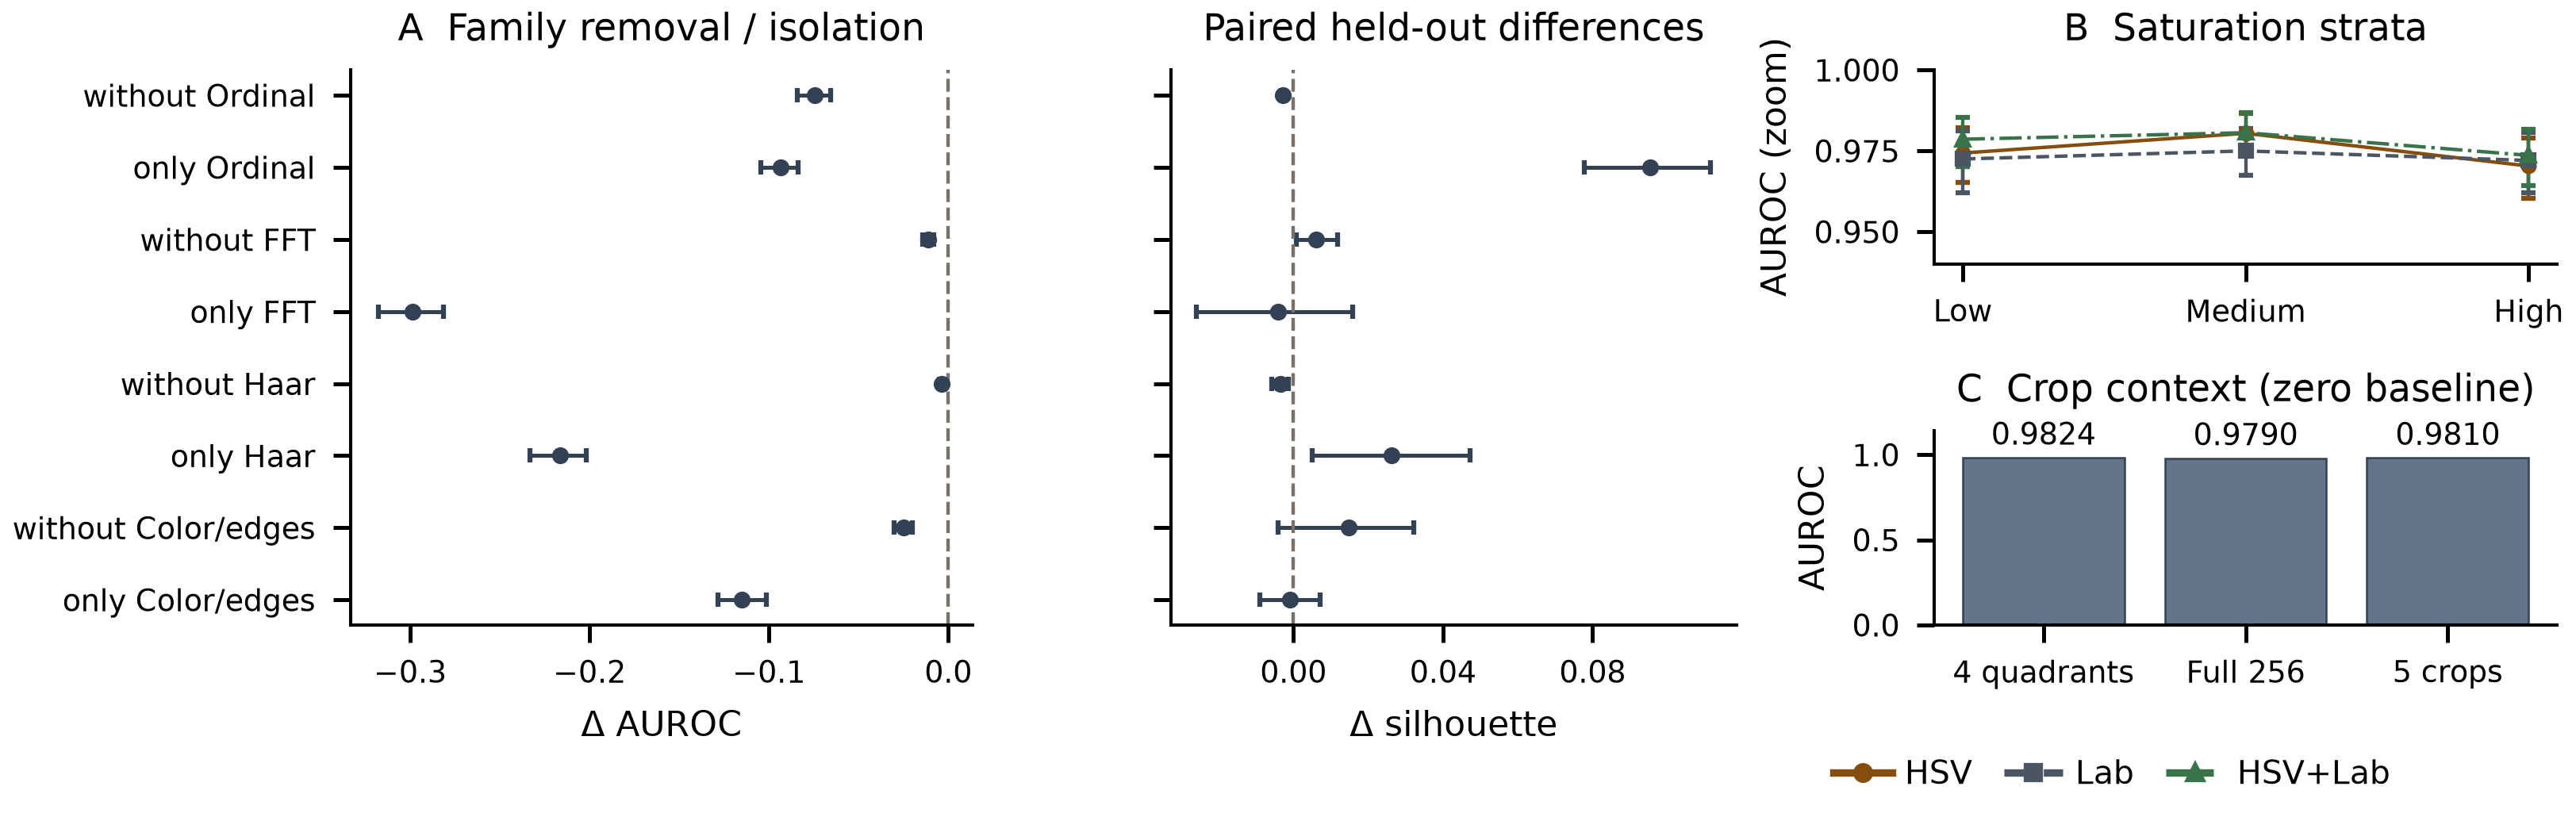
\includegraphics[width=\textwidth,height=2.3in,keepaspectratio]{figure_10.png}

\caption{Paired family losses and color/crop sensitivities; ordinal removal causes the largest conditional AUROC decrease. B retains all intervals on an explicitly zoomed axis; C bars start at zero. Group intervals retain fits; silhouette intervals additionally retain geometry.}\label{fig:f10}

\end{figure*}
HSV, Lab and their combination vary across development-defined saturation tertiles. Strata remain descriptive. Tie exclusion reduces AUROC to 0.9753. Full-$256^2$ and five-overlapping-$128^2$-crop variants reach 0.9790 and 0.9810, respectively. The full-image variant also changes predictor dimensionality, so the difference cannot be attributed solely to context size. Group-paired intervals condition on frozen fits; silhouette intervals additionally condition on cached geometry.
\subsection{JPEG Recompression and Resizing}
Both origins undergo identical transformations with the primary probe and scaler frozen. Table~\ref{tab:t10} and Fig.~\ref{fig:f11} show AUROC 0.9822 at JPEG 95, 0.8354 at JPEG 75 and 0.6819 at JPEG 50. The latter retains only style-rank Spearman $\rho=0.3697$, while full-space origin-silhouette retention increases to 1.3749. Bilinear downsampling to 128 and upsampling to 256 before feature extraction yields AUROC 0.7744. Silhouette ratio divides mean full-space origin silhouette by its original value; $\rho$ correlates ten styles ranked by mean standardized $W_1$ over 104 features. Ranking and geometric separation respond differently. Original inputs are release JPEGs, not pristine quality-100 images. Equal recompression cannot restore absent subject correspondence or encoding support. No equal-encoding retraining was run; stress tests retain the original fitted probe.
\begin{table*}[t]
\caption{Frozen-probe stress tests. AUROC-difference intervals are paired group-bootstrap 95\% intervals; original inputs are release JPEGs.}\label{tab:t10}
\centering\footnotesize
\setlength{\tabcolsep}{3pt}\renewcommand{\arraystretch}{1.10}
\begin{tabularx}{\textwidth}{>{\hsize=0.960\hsize\linewidth=\hsize\raggedright\arraybackslash}X>{\hsize=0.720\hsize\linewidth=\hsize\raggedright\arraybackslash}X>{\hsize=0.720\hsize\linewidth=\hsize\raggedright\arraybackslash}X>{\hsize=1.800\hsize\linewidth=\hsize\raggedright\arraybackslash}X>{\hsize=0.900\hsize\linewidth=\hsize\raggedright\arraybackslash}X>{\hsize=0.900\hsize\linewidth=\hsize\raggedright\arraybackslash}X}
\toprule
\textbf{View} & \textbf{AUROC} & \textbf{F1} & \textbf{95\% CI} & \textbf{Silhouette ratio} & \textbf{Rank $\rho$}\\\midrule
{}jpeg95 & 0.9822 & 0.9430 & [-0.0003, -0.0000352] & 0.9922 & 1.0000\\
{}jpeg75 & 0.8354 & 0.7453 & [-0.1586, -0.1347] & 0.9639 & 0.9636\\
{}jpeg50 & 0.6819 & 0.6921 & [-0.3170, -0.2832] & 1.3749 & 0.3697\\
{}resize0.5 & 0.7744 & 0.6772 & [-0.2244, -0.1918] & 0.8420 & 0.8788\\
{}resize0.75 & 0.8325 & 0.6986 & [-0.1631, -0.1366] & 0.8649 & 0.9030\\
\bottomrule\end{tabularx}
\end{table*}
\begin{figure*}[t]

\centering

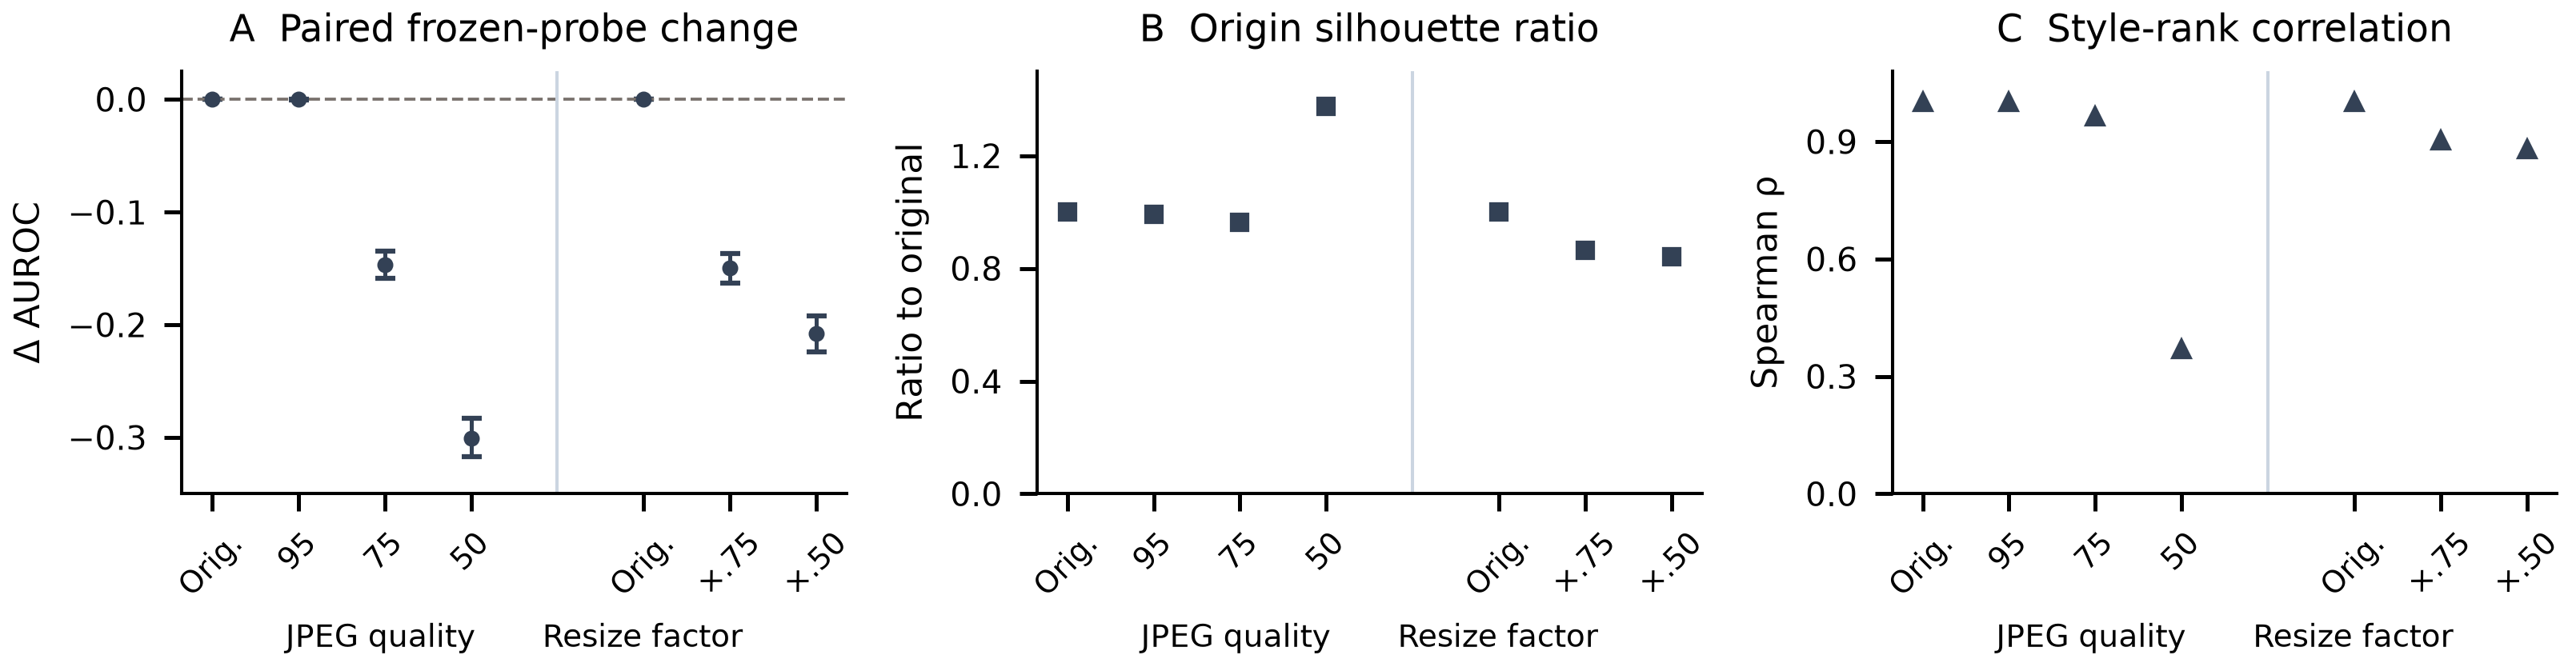
\includegraphics[width=\textwidth,height=1.85in,keepaspectratio]{figure_11.png}

\caption{Separate panels and condition groups avoid dual-axis ambiguity. A shows paired AUROC changes and group-bootstrap 95\% intervals from Table XII; original is the zero reference. B/C are descriptive point estimates without computed intervals; ranks use ten styles. JPEG 50 reduces ranking despite increased silhouette.}\label{fig:f11}

\end{figure*}

\section{Discussion}
\subsection{Common-Support Failure and Technical Source Association}
ResNet-50 and DINOv2 outperform the handcrafted probe, but ranking release labels differs from attributing differences independently of subjects and processing. The common-support gate (Algorithm~\ref{alg:pipeline}, line 8) blocks that stronger inference: origin-aligned JPEG quantization and unverified subjects invalidate interpreting 542 exploratory passes as confirmed diffusion-origin effects, without erasing their descriptive associations.

Whole-group permutations preserve recorded families, not verified exchangeability. Multiplicity adjustment and frozen-fit bootstrap intervals cannot remove confounding or create common support. Zero of 1,040 comparisons is confirmed because none is eligible, not because each null is accepted; neither zero true effects nor complete JPEG mediation follows. An untested hypothesis is that ordinal patterns respond to JPEG blocks and thereby contribute to the largest ablation effect; JPEG-50 sensitivity motivates, but does not establish, this mechanism.

\subsection{Forensic Cases and Boundary Sensitivity}
Table~\ref{tab:t11} indexes two FP, two FN, two TP and two H--C/PCA outliers. Figure~\ref{fig:f12} connects actual canvases and quadrants to their measurements. Typographic cards, ornate frames, isolated objects and monochrome examples illustrate unusual inputs, without verified semantic/material annotation. The cases are purposive and restricted to the primary Human--LD test; no SD-specific error-gallery arm was run.
\begin{table*}[tb]
\caption{Purposively selected held-out cases. IDs are prefixes; complete IDs and measurements accompany the paper.}\label{tab:t11}
\centering
\footnotesize
\setlength{\tabcolsep}{3pt}
\renewcommand{\arraystretch}{1.12}
\begin{tabularx}{\textwidth}{>{\hsize=1.202\hsize\linewidth=\hsize\raggedright\arraybackslash}X>{\hsize=0.919\hsize\linewidth=\hsize\raggedright\arraybackslash}X>{\hsize=0.636\hsize\linewidth=\hsize\raggedright\arraybackslash}X>{\hsize=1.414\hsize\linewidth=\hsize\raggedright\arraybackslash}X>{\hsize=0.990\hsize\linewidth=\hsize\raggedright\arraybackslash}X>{\hsize=0.919\hsize\linewidth=\hsize\raggedright\arraybackslash}X>{\hsize=0.919\hsize\linewidth=\hsize\raggedright\arraybackslash}X}
\toprule
\textbf{ID} & \textbf{Case} & \textbf{origin} & \textbf{style} & \textbf{p(AI)} & \textbf{H} & \textbf{C}\\\midrule
{}2f0c78f46f & FP & Human & renaissance & 1.0000 & 0.9870 & 0.0168\\
{}305d3cd479 & FP & Human & surrealism & 0.9998 & 0.8614 & 0.1551\\
{}e679eb4f82 & FN & LD & realism & 0.0010 & 0.9168 & 0.1036\\
{}6c9f139321 & FN & LD & expressionism & 0.0254 & 0.9567 & 0.0560\\
{}f3fa732e66 & TP & LD & art\_nouveau & 1.0000 & 0.9086 & 0.1160\\
{}89f0f4d605 & TP & LD & baroque & 1.0000 & 0.9498 & 0.0667\\
{}f4af268f19 & HC outlier & Human & art\_nouveau & <0.00000001 & 0.4618 & 0.2216\\
{}a1dce1b036 & PCA outlier & Human & romanticism & 0.00000968 & 0.9773 & 0.0287\\
\bottomrule\end{tabularx}
\end{table*}
\begin{figure*}[t]

\centering

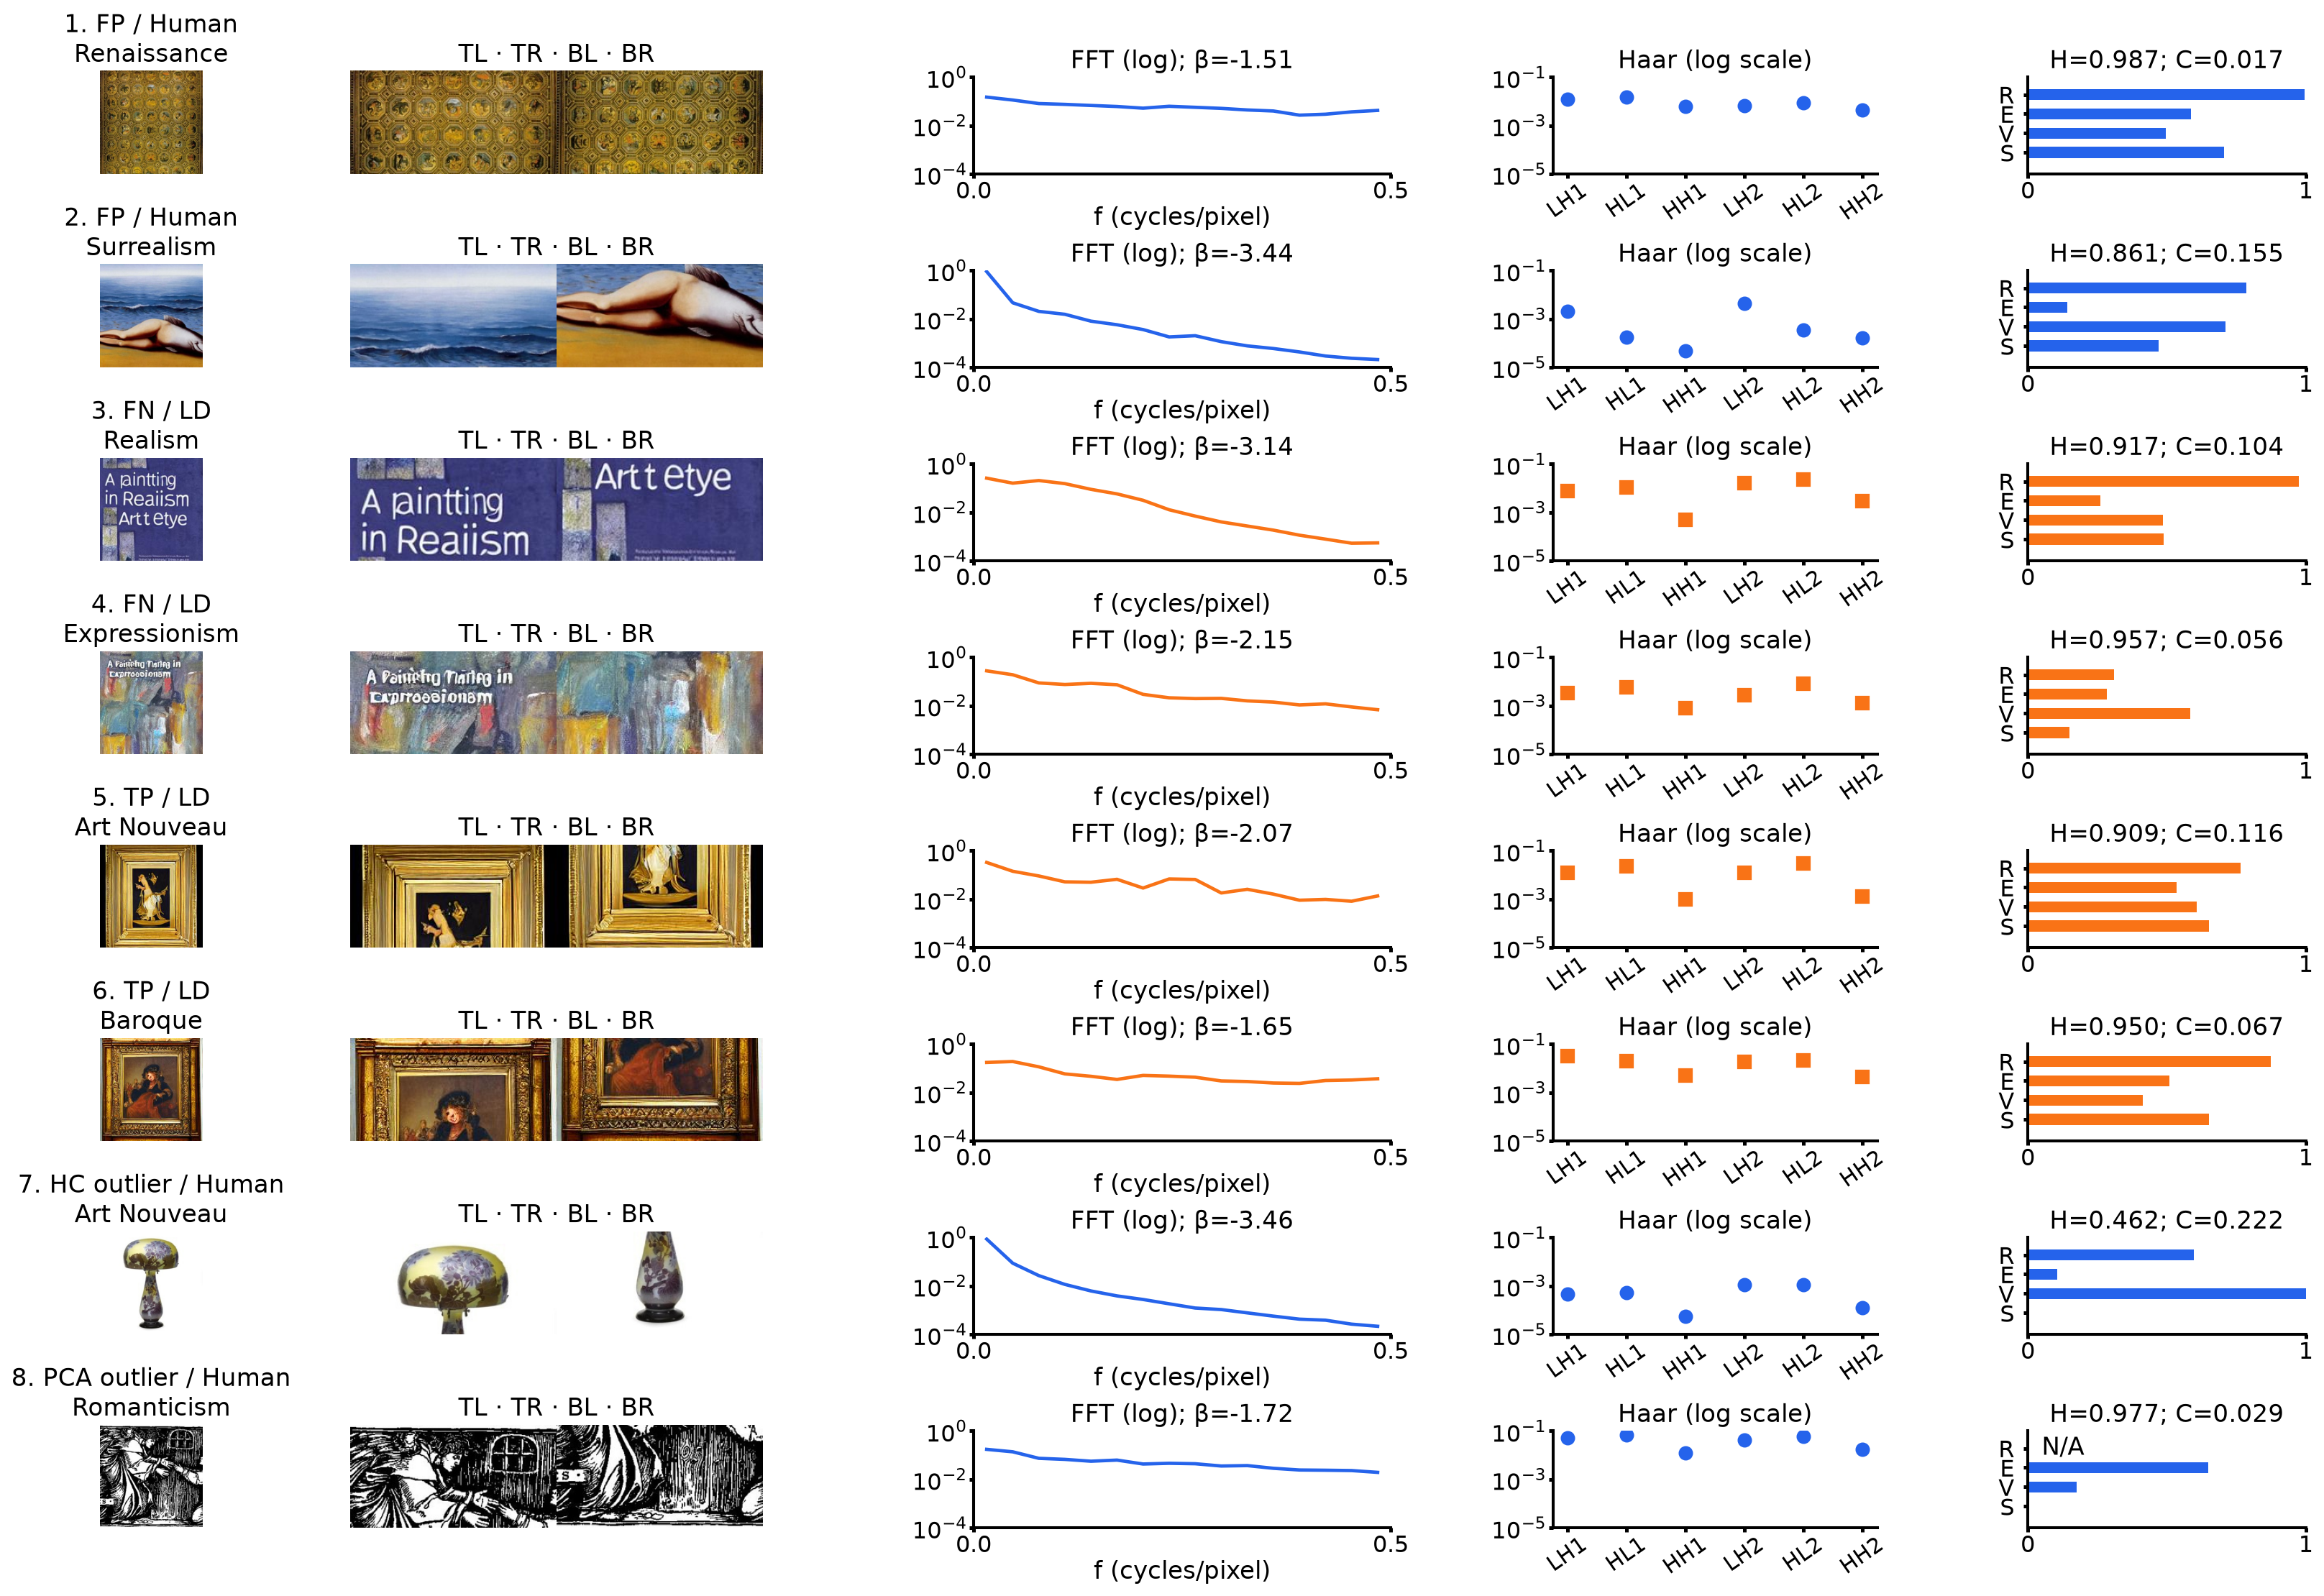
\includegraphics[width=\textwidth,height=4.9in,keepaspectratio]{figure_12.png}

\caption{Eight purposive cases, not prevalence estimates; FP/FN/TP refer to release labels. FFT rows share 10$^{-4}$--1 and Haar rows 10$^{-5}$--10$^{-1}$, both logarithmic. S = saturation, V = value, E = edge density, R = hue concentration (N/A when undefined).}\label{fig:f12}

\end{figure*}
Development-defined saturation/edge/frequency proxies complement a fixed border heuristic (released \texttt{src/border\_analysis.py}). It flags 369 artworks; 76 lose every quadrant. The identical 5,924 supported artworks yield 12 signed-shift and 23 exploratory-rule reversals, with zero confirmed reversals. Support sensitivity does not repair subject/encoding controls. Overlapping-trigger error gaps and group intervals are in \texttt{failure\_trigger\_associations.csv}.

\subsection{Threats to Validity and Gap Verdicts}
\textit{Internal validity:} deterministic encoding differences, unavailable verified subjects and uncertain AI filename-family semantics prevent independent origin attribution. Known Human artist groups are protected, but unknown derivative links can remain.

\textit{External validity:} ten release movements and two primary origins are tested; SD resizing and mixed-source composition restrict transfer, with no separate artist/style/generator holdouts.

\textit{Construct validity:} entropy, complexity and color are formal descriptors, not aesthetic merit or intentional style. Quantile triggers are proxies, and an inspectable dashboard has no user-study validation. G1 is addressed through implemented diagnostics (auditability and measured fidelity); explanation faithfulness and human usefulness were not tested, and display PCA trustworthiness is 0.6928. G2 is achieved descriptively over the 1,040 feature/style cells, not as temporal art-history inference.

\textit{Statistical conclusion validity:} source dependence reduces effective sample size; conditional bootstraps and unsupported randomization exchangeability restrict interpretation. Resampling precision cannot substitute for matched subjects. G3 yields a negative validity audit consistent with encoding leakage; the original requirement that separation survive verified controls remains unestablished.

\section{Conclusion and Future Work}
The control-gated workflow joins named features, grouped probes, projection diagnostics and linked artwork evidence. Strong release prediction coexists with origin-aligned encoding and unverified subjects; within-style shifts remain descriptive. Frozen ResNet-50 and DINOv2 outperform the handcrafted probe, but none establishes encoding-independent attribution. Future work requires common-encoding originals, verified subject/prompt links and separate artist/style/generator holdouts. Independent annotations and human evaluation are needed to test material-specific explanations and dashboard usefulness.

\section{Declarations and Acknowledgements}
\textit{Data and code availability:} AI-ArtBench is available from its authors\footnote{\url{https://www.kaggle.com/datasets/ravidussilva/real-ai-art}} \cite{p1}; ArtBench-10 supplies its human-art source \cite{artbench}. The prepared local release contains code/tests, pinned dependencies, frozen split IDs/cohort hash, CSVs, figure generators and build commands; the original release is public; this audited revision requires an updated commit. Raw images, model weights and large caches are excluded. The official code and artifact repository is \url{https://github.com/wasil-7/explainable-diffusion-art-analytics}. No fresh-environment experimental replication is claimed.

\textit{Competing interests and funding:} The authors declare no competing interests. This research received no external funding. \textit{AI-assisted tools:} Codex, Antigravity, Claude and SciSpace supported coding, literature exploration, drafting and formatting. Wasil Kayani and Umar Asghar verified the evidence and take responsibility for the final manuscript. \textit{Acknowledgements:} The authors thank Ms. Azka Atiq and FAST National University of Computer and Emerging Sciences (FAST-NUCES), Islamabad, for academic guidance.

\bibliographystyle{IEEEtran}
\bibliography{references}
\appendices
\section{Compact Reproducibility Summary}
{\footnotesizeFrozen cohort SHA256: \texttt{e27a00766ad8825201aac6d4167a5a98b}\allowbreak\texttt{319d5b18b136ffb20d5765073472936}.

Unweighted L2 L-BFGS: max\_iter 2000, tol $10^{-4}$. PCA: three components/full SVD. t-SNE: random initialization, automatic learning rate, 1,000 iterations, perplexities 15/30/50. NumPy Lloyd: k=2, k-means++, 20 starts, maximum 300 iterations.

CUDA 12.4, driver 621.14; cuDNN unrecorded. Fit/tune s (Table~\ref{tab:t4}): 7.00, 0.47, 0.11, 12.49, 1.70. ResNet-50/DINOv2 partial cache timings: 2916.85/5020.19 s; cold imports/interruptions excluded. $C_{\mathrm{solver}}$ (Table~\ref{tab:t4} order): 10, 10, 0.001, 1, 1. Thresholds: 0.4380, 0.4036, 0.6415, 0.7827, 0.2774.
}
\end{document}
